% !!!!!!!!!!!!!!!!!!!!!!!!!!!!!!!!!!!!!!!!!!!!!!!!!!!!!!!!!!!!!!!!!!!!!!!!!!!!
%                                                                            !
% Adapt this file so that you can use it for your thesis					 !
%                                                                            !
% !!!!!!!!!!!!!!!!!!!!!!!!!!!!!!!!!!!!!!!!!!!!!!!!!!!!!!!!!!!!!!!!!!!!!!!!!!!!


\documentclass{micro-econ-thesis}
\usepackage{graphicx}
\usepackage{setspace}
\usepackage{float}
\usepackage[utf8]{inputenc} % depends on the font encoding that you are using

% For formatting of your bibliography, please use the following package with options 
\usepackage[style=authoryear]{biblatex}
\usepackage{gensymb}
\usepackage{amsmath}
\usepackage{booktabs}

\usepackage{chngcntr}
\counterwithout{table}{section}

\addbibresource{bibliography.bib} % add a bib-reference file

\begin{document}
% ----------------------------------------------------------------------------
% Details for the titlepage
% ----------------------------------------------------------------------------
\thesisTitle{Development of Analysis Techniques for dynamic magnetic resonance imaging}
\thesisType{Master Thesis} % 'Master Thesis' or 'Seminar Paper'
\thesisAuthor{Aayush Nepal}
\thesisMail{aayush.nepal@uni-jena.de}
\thesisGrade{Master of Science in Medical Photonics} % leave empty for seminar papers
\thesisTutora{Prof. Dr. rer. nat. med. habil. Jürgen Reichenbach}
\thesisTutorb{Dr. rer. nat. Martin Krämer}
\thesisMatrikel{198683}
\thesisAddress{Schützenggase 2\\[.5ex]
								99423 Weimar}
\thesisDate{\today}
% In case of external supervisor
\thesisCompany{}

% Print titlepage
\thesisMakeTitle

% ----------------------------------------------------------------------------
% Abstract
% ----------------------------------------------------------------------------
\cleardoublepage
\pagenumbering{roman}
\pagestyle{plain}
%\thispagestyle{empty}
\subsection*{Abstract}


\clearpage
\subsection*{Acknowledgements}


% ----------------------------------------------------------------------------
% Table of contents
% ----------------------------------------------------------------------------
\cleardoublepage
%\thispagestyle{empty}
\tableofcontents

% ----------------------------------------------------------------------------
% List of figures/tables
% ----------------------------------------------------------------------------
\cleardoublepage
\phantomsection
\addcontentsline{toc}{section}{List of Figures}
\listoffigures
% --------------------------
\cleardoublepage
\phantomsection
\addcontentsline{toc}{section}{List of Tables}
\listoftables
% --------------------------

\cleardoublepage
\phantomsection
\addcontentsline{toc}{section}{List of Acronyms}
\section*{List of Acronyms}
\begin{tabular}{@{}ll}
FSU Jena & Friedrich-Schiller-Universität Jena\\
\end{tabular}

% --------------------------

% ----------------------------------------------------------------------------
% Contents
% ----------------------------------------------------------------------------
\cleardoublepage
\pagestyle{headings}
\pagenumbering{arabic}
\setcounter{page}{1}
% Contents
\onehalfspacing % for linespacing 1.5, you can turn it off with \singlespacing, e.g. for quotes or tables with multiline cells

\section{Introduction}

This thesis investigates the biomechanical analysis of the knee joint using high-resolution CINE MRI imaging, focusing on the dynamic interactions between the femur and tibia during flexion-extension cycles under various loading conditions. With advancements in MRI technology, detailed images of knee movements can be captured, which presents unique opportunities for extracting meaningful insights into invivo knee dynamics that can contribute to orthopedic research and clinical practice.

The primary challenge in utilizing these detailed images lies in the accurate segmentation of key anatomical structures. This segmentation is crucial, as it significantly influences the reliability of biomechanical measurements derived from the MRI data. Traditional manual segmentation methods, while straightforward, are time-consuming and prone to inconsistencies, especially when dealing with multiple frames across time. To address these issues, this thesis proposes the development of a semi-automated segmentation pipeline. This new methodology aims to streamline the segmentation process, reducing the time and effort involved while enhancing accuracy and consistency across sequential images.

Following the successful segmentation of the femur and tibia, the subsequent analysis involves quantifying two distinct biomechanical parameters: the angle between the long axes of the segments and the distance between specific anatomical landmarks on these bones. These measurements are calculated from single-slice 2D images in sagital view captured throughout the knee's motion cycle under both loaded and unloaded conditions. The purpose of this quantification is to explore potential differences in the kinematics of the knee joint under varying load and to provide an indirect assessment of joint space and functionality.




\section{Fundamentals}
\label{sec:intro}


\subsection{The Knee Joint }
The knee joint, a pivotal structure in the human body, plays an essential role in locomotion. Additionally, it functions to control the center of body mass and posture in the activities of daily living by facilitating a wide range of movements. As such, the knee's health and integrity are vital for overall quality of life, influencing everything from basic mobility to participation in complex sports. A comprehensive survey across 15 European countries and Israel found that knee pain was the third most commonly reported type of chronic pain. This underscores the significant public health concern it represents \parencite{breivik_survey_2006}. Furthermore, arthritis/osteoarthritis (OA) was identified as the most common cause of this pain. 

This situation has not improved over time. In Germany for instance, a recent retrospective study has found that the number of patients with OA is steadily rising \parencite{obermuller_epidemiology_2024}. 
Knee-related issues are prevalent and impactful due to the inherent complexity of the knee joint itself. As a hub of various anatomical structures working in unison, the knee supports a range of movements and bears significant loads, making it susceptible to a variety of injuries and conditions.
Understanding the anatomy of the knee is the first step in tackling this problem. 

\textbf{Anatomy and Function}

The knee joint is the largest and the most superficial synovial joint in the body. \parencite{dalley_moores_2023}. 
It comprises three primary articulations:two femorotibial articulations (see Figure \ref{fig:rightkneeplate519}) and one femoropatellar articulation. These articulations, illustrated in Figure \ref{fig:rightkneeplate519} and \ref{fig:patellarsurface}, are defined by their complexity and incongruence, features that are crucial for the joint's biomechanical performance. 
 
\begin{figure}[H]
	\centering
	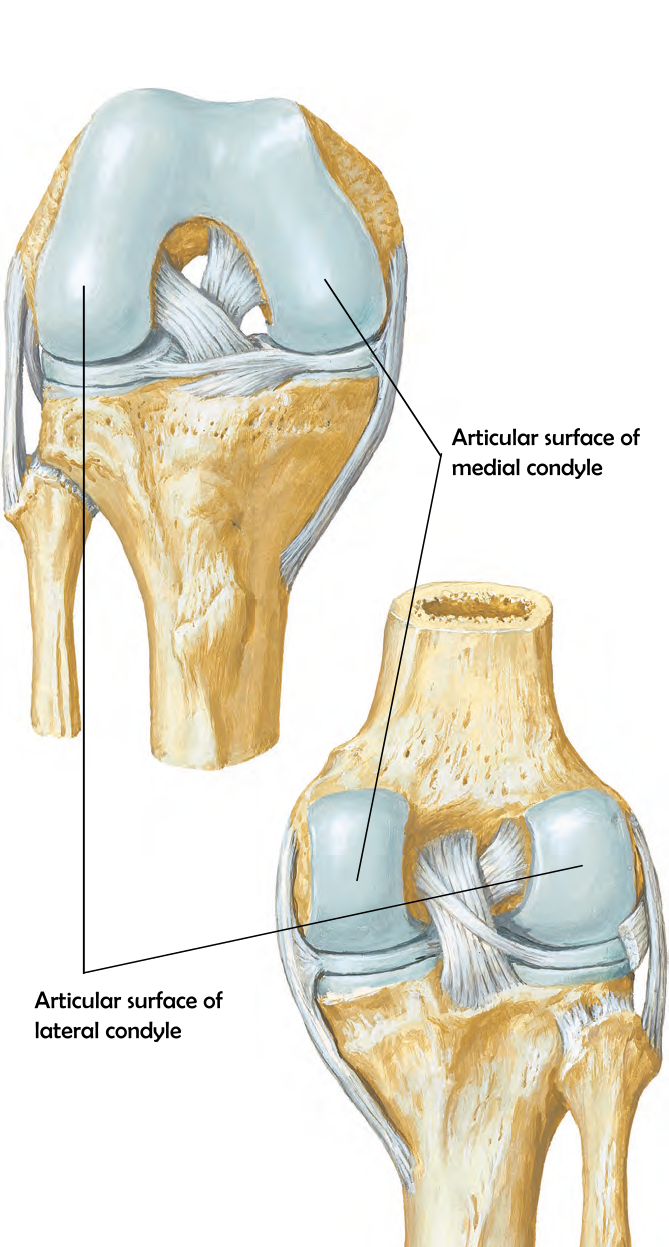
\includegraphics[scale=0.3]{right_knee_labeled}
	\caption{Anterior (flexed,top) and posterior (extended, bottom) view of the right knee with their articular surfaces labeled. [Edited] \parencite[p.519]{netter_519_2023}}
	\label{fig:rightkneeplate519}
\end{figure}

\begin{figure} [H]
	\centering
	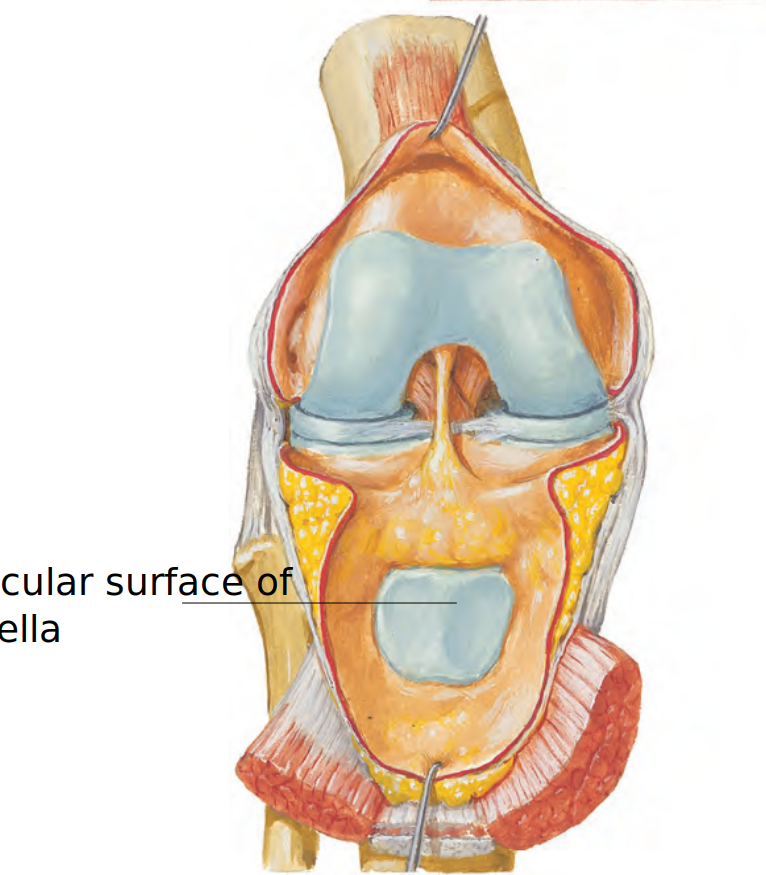
\includegraphics[scale=0.3]{patellar_surface}
	\caption[patellar surface]{Right joint opened, knee slightly in flexion, with the patellar articulation labelled. [Edited] \parencite[p.517]{netter_519_2023}}
	\label{fig:patellarsurface}
\end{figure}

This design allows the knee to manage a wide array of movements and bear significant loads. Figure \ref{fig:sixdegrees} illustrates the knee's capacity for multidimensional movement, highlighting the joint's sophisticated structural design that enables this versatility. However, this inherent design also renders the knee vulnerable to a range of forces \parencite{standring_grays_2021}.

\begin{figure}[H]
	\centering
	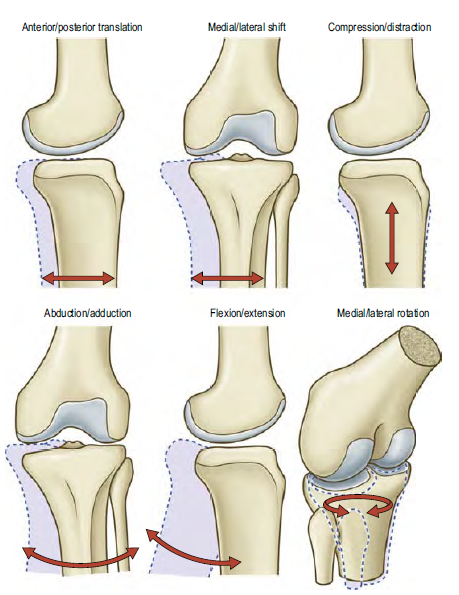
\includegraphics[width=0.7\linewidth]{six_degrees}
	\caption{The knee joint motion in three dimensions, described using six independent variables (degrees of freedom) \parencite[p.~1412]{standring_grays_2021}.}
	\label{fig:sixdegrees}
\end{figure}

Such mechanical forces, influenced by activities and body mass index (BMI), are significant causes of OA and represent one of the most modifiable risk factors \parencite{heidari_knee_2011}. Furthermore, abnormal joint loading is considered a key mechanical driver of osteochondral changes thought to contribute to the initiation and progression of knee OA \parencite{coburn_immediate_2023}.


The relationship between biomechanical stresses and knee health highlights the need for diagnostic tools that fulfill two key criteria: they must capture the knee's dynamic behavior during motion and assess the joint under varying loads. Dynamic magnetic resonance imaging (MRI) excels in meeting these requirements as one of the most advanced imaging modalities.


\subsection{Dynamic MRI}
In a broad sense, dynamic MRI is an umbrella term encompassing various MRI techniques designed to capture and visualize physiological processes and motion over time. The dynamic aspect of MRI is crucial for studying systems or structures involving inherent motion, such as blood flow, tissue perfusion, or cardiac activity. For the purposes of this project, the focus of "dynamic MRI" narrows down to capturing the bulk movement of the knee joint undergoing active flexion extension cycles inside the scanner. Compared to traditional static MRI scans, which are highly susceptible to motion artifacts compared to other imaging modalities \parencite{zaitsev_motion_2015}, dynamic MRI techniques not only accommodates motion, but can even leverage it to offer comprehensive insights into the functional and biomechanical properties of the concerned structures.  Among these techniques, CINE imaging, particularly renowned in cardiac MRI, is considered the gold standard for evaluating cardiac function \parencite{menchon-lara_reconstruction_2019}. Its high regard in cardiac MRI demonstrates the method's precision and adaptability—traits that are leveraged in knee imaging.

\subsubsection{CINE imaging}

CINE, derived from 'cinematography,' refers to creating a movie-like sequence of images. In the context of dynamic knee MRI, this technique can be used to reconstruct a "movie" of a single flexion-extension cylce. This visualization is achieved by aggregating multiple partial datasets acquired over various cycles. The knee's movement cycle is segmented into distinct stages, each corresponding to a specific angle of flexion or extension. For each stage, k-space — the Fourier transform space from which MR images are reconstructed — is incrementally sampled. This data is gathered across multiple repetitions of the movement cycle, ensuring comprehensive coverage of k-space and thus, high-resolution imaging of each movement phase.This technique works robustly only if the movement cycles of the knee during imaging are sufficiently similar to each other \parencite{curtis_primer_2022}. Achieving this consistency in dynamic MRI of the knee, which naturally involves significant movement variations, requires precise synchronization of the imaging process with the knee's motion cycle. 

\subsubsection{Gating} 

This synchronization, known as gating, aligns image acquisition with specific, repeatable points in the knee's movement cycle. By ensuring each captured image corresponds accurately to a consistent phase of motion, it minimizes the discrepancies that can arise from cycle-to-cycle variations, enhancing the reliability of bio-mechanical analyses. Retrospective gating, one of the two main types alongside prospective gating, provides consistent image quality. This makes it a suitable choice for applications like CINE imaging \parencite[p. 102]{edelman_clinical_1996}. In retrospective gating, the data is acquired continuously throughout the motion cycle. The data is then reordered post-acquisition into a coherent sequence that shows the knee at different positions along the motion cycle. This necessitates external information that captures the precise moment and position of the knee throughout its range of movement beyond just the raw data acquired during the MRI scan. A previously reported novel knee loading device is employed to address this, which comes with an optical sensor attachment that provides this vital information. This sensor provides information that includes the exact timing and degree of knee flexion and extension, which is essential for accurately synchronizing the imaging frames with specific phases of the knee’s motion cycle \parencite{brisson_novel_2022}. 

\subsubsection{Knee loading device }

The MR-compatible knee loading device employed in this study is illustrated in Figure \ref{fig:kneedevice}. This device allowed for a range of motion of approximately 25 to 45 degrees (subject-dependent), enabling subjects to perform knee flexion and extension cycles under both loaded and unloaded conditions. For loading, the device was equipped with compartments for weight plates and sandbags, providing a physiological load of 10 to 12 kilograms. These weights are positioned at the distal end of the device, directly influencing the mechanics of knee extension. As the subject extends the knee, they must overcome not only the natural resistance of their body weight but also the additional external load imposed by these weights. Central to this device's functionality is an optical fiber position sensor (MR338-Y10C10, Micronor, 155 Camarillo, CA, USA), which precisely  measures the ab­solute angle from 0{\degree}\,to 360\degree \, with a resolution of 0.025\degree \parencite{rickenbach_optical_2013}. This measurement capability is critical for synchronizing the knee's movement with MRI data reconstruction. 
\begin{figure} [H]
	\centering
	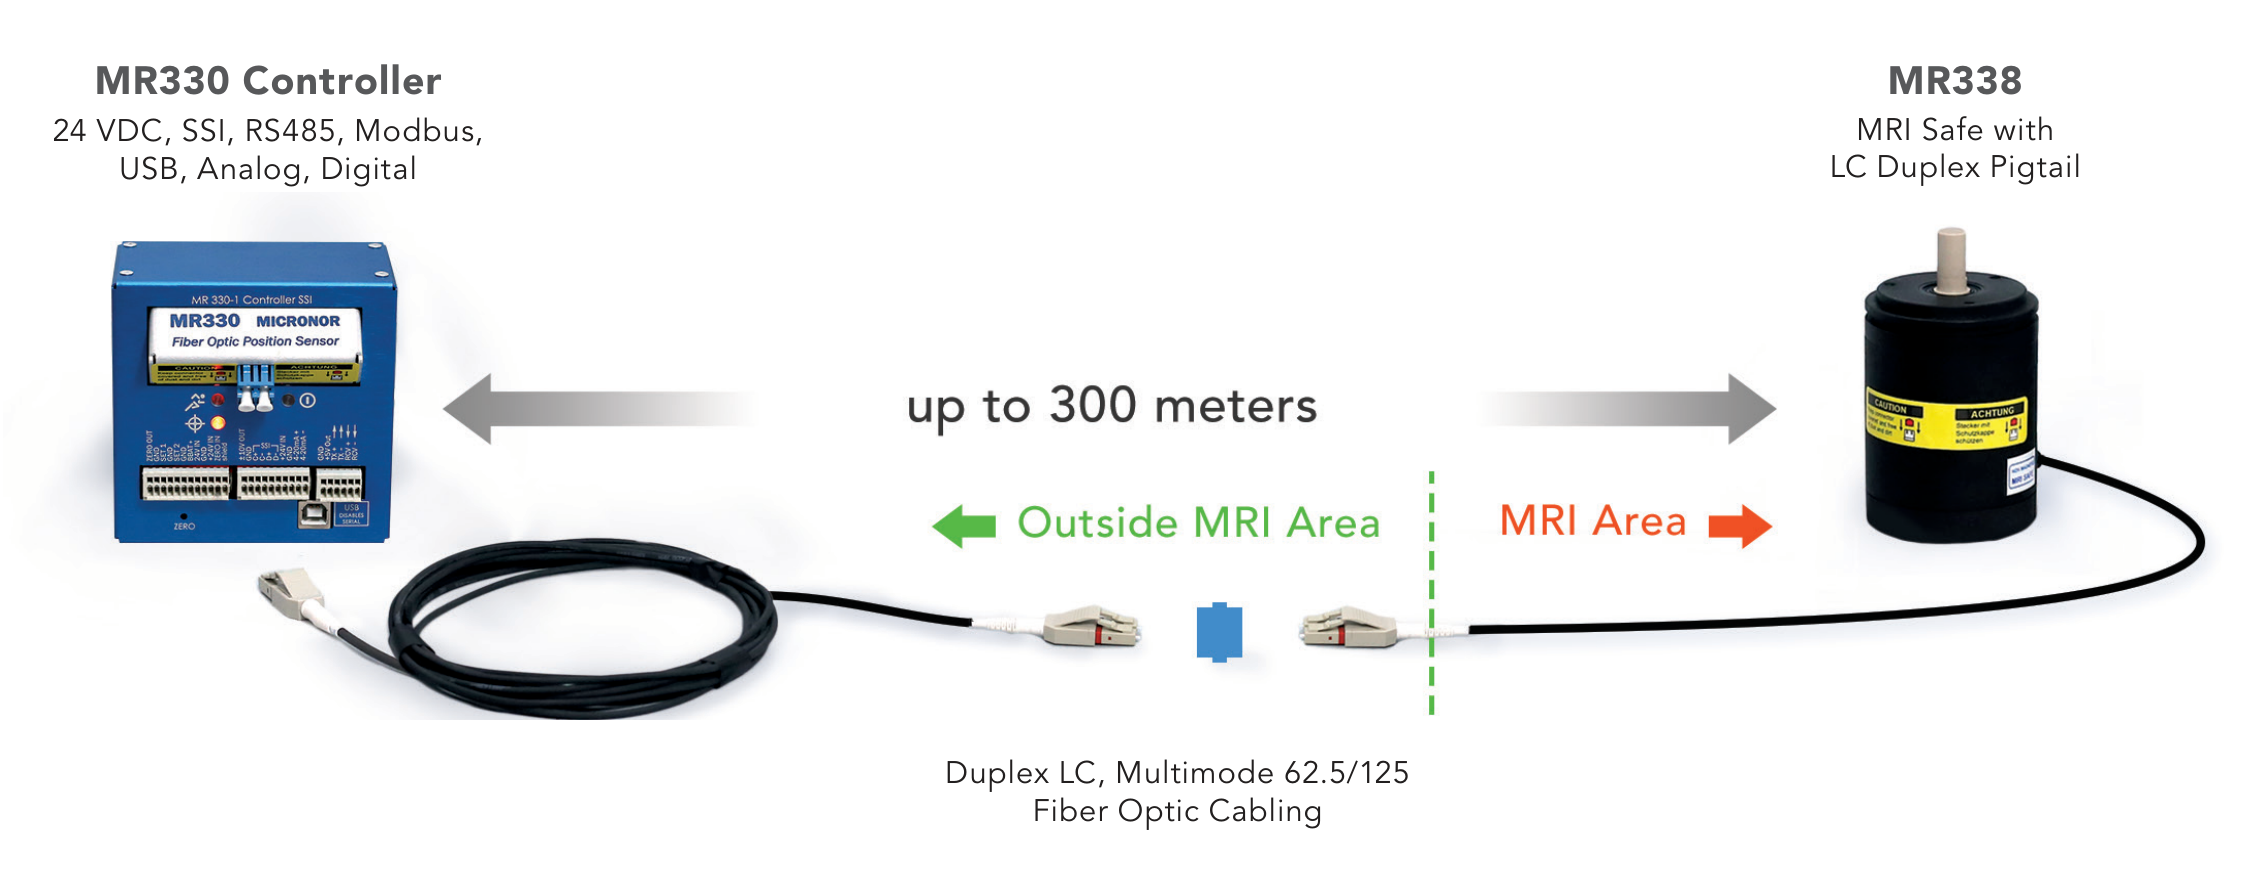
\includegraphics[width=0.7\linewidth]{sensor_img}
	\caption{The MR330 controller (left) and MR338 optical fiber position sensor system (right), showcasing the connection from the controller to the sensor via duplex LC multimode fiber optic cabling.}
	\label{fig:sensorimg}
\end{figure}


As shown in Figure \ref{fig:sensorimg} , the MR330 controller interfaces with the MRI-safe MR338 position sensor to facilitate precise measurement within the MRI environment, accommodating up to 300 meters of fiber optic cabling. The controller is connected to a acquisition computer placed outside the scanner while the sensor is attached to the device within. To enhance signal acquisition and the clarity of imaging, two flexible coils \underline{(cite the coils here, perhaps also show a picture)} were positioned at key anatomical locations: one at the distal femur and another at the proximal tibia, as specified in the MRI protocol.
\begin{figure}[H]
	\centering
	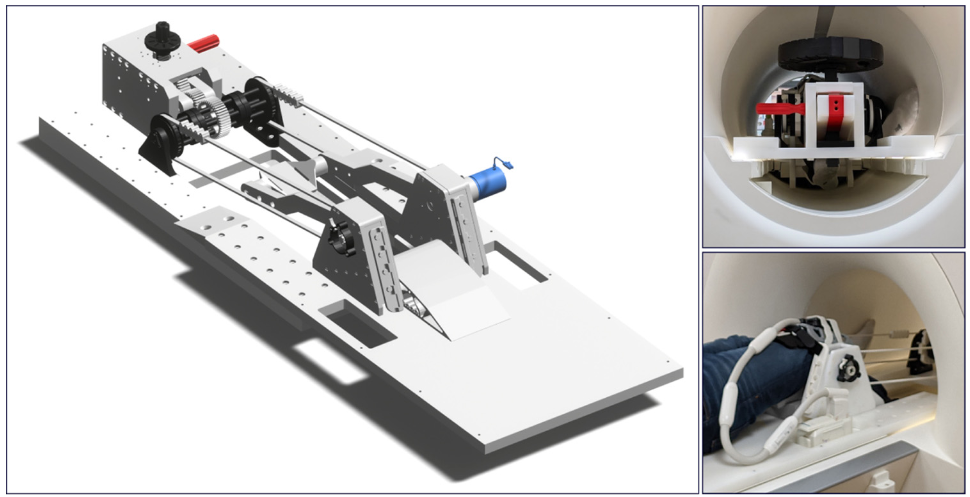
\includegraphics[width=0.9\linewidth]{knee_device}
	\caption{A 3D rendering of the knee motion/loading device (left) and two photographs of the device in a Siemens Magnetom Prisma Fit MRI scanner (right). The top right image (rear view) demonstrates how the distal part of the device sits atop the rails within the scanner bore, which are normally used to guide and support the patient table. The bottom right image (front, oblique view) demonstrates an individual positioned in the device with a flexible coil around the index knee, the thigh secured between the proximal pillow blocks and the ankle fastened to the leg support, as well as the coil plug setup \parencite{brisson_novel_2022}. }
	\label{fig:kneedevice}
\end{figure}
 


  
To further enhance the quality and precision of our imaging, and to maximize the potential for precise image reconstruction, a previously reported radial golden-angle gradient-echo FLASH sequence was used, which is more robust against motion artifacts than Cartesian sequences \parencite{aleksiev_high-resolution_2022}. The following sections will detail the key components of this technique — radial golden-angle acquisition and the gradient-echo FLASH sequence.

\subsubsection{Radial golden-angle acquisition}


As the name suggests, radial golden-angle acquisition specifically modifies how k-space is sampled. Unlike traditional static MRI, which typically employs Cartesian sampling, this method utilizes radial sampling. Here, the data points are collected along radial lines spreading out from the center of k-space, resembling spokes on a wheel. Figure \ref{fig:radial} depicts a generic radial sampling scheme. The separation between any two adjacent circles defines the separation $\Delta k_r$ in the radial sampling direction, whereas, the angular separation between any two successive angular lines in k-space (such as between the two example lines shown in the figure) defines $\Delta \theta$. The two quantities $\Delta k_r$ and $\Delta \theta$ are constrained by the Nyquist sampling criterion. \parencite{brown_magnetic_2014} 
  
 \begin{figure}[H]
 	\centering
 	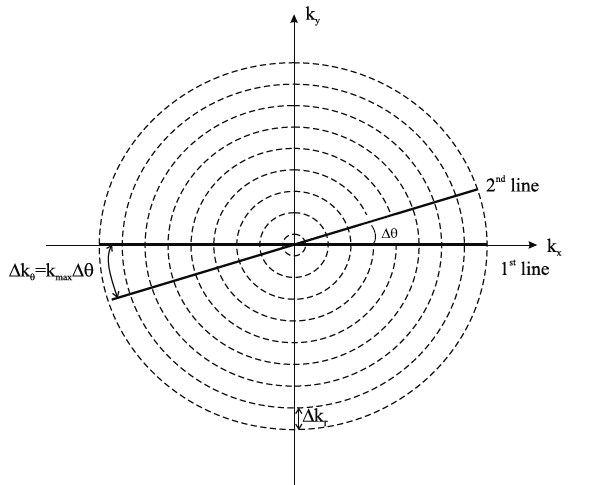
\includegraphics[width=0.7\linewidth]{radial}
 	\caption{Generic radial k-space sampling \parencite[p.306]{brown_magnetic_2014}}
 	\label{fig:radial}
 \end{figure}
 
 The 'golden-angle' strategy, which we employ, optimizes this approach by spacing the radial lines at an angle of approximately 111.25 degrees. This specific angle helps in evenly covering the k-space without overlapping, ensuring that each new image frame provides unique information, thus enhancing image quality and temporal resolution. 
 
\begin{figure}[H]
	\centering
	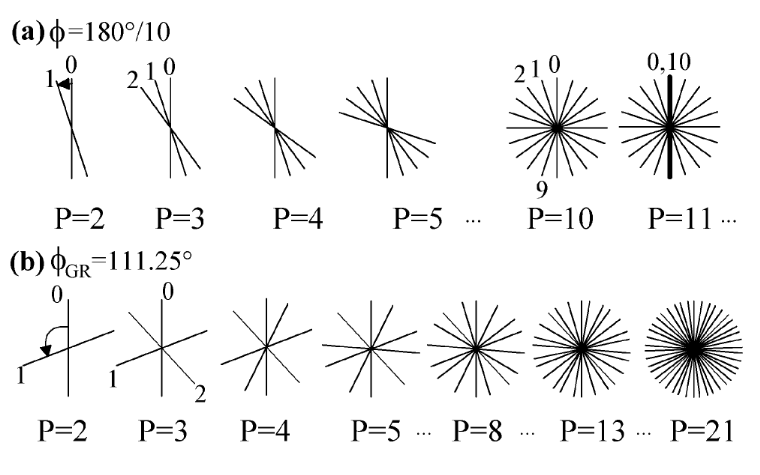
\includegraphics[width=0.7\linewidth]{golden_angle_figure}
	\caption{Radial k-space sampling strategies. (a) Fixed angular increment, showing potential for uneven k-space coverage. (b) Golden-angle sampling, ensuring uniform distribution across k-space \parencite{winkelmann_optimal_2007}.}
	\label{fig:goldenanglefigure}
\end{figure}

 
Figure \ref{fig:goldenanglefigure} provides a visual comparison between traditional fixed increment and the golden-angle methods in k-space sampling. It highlights how each approach affects the distribution of sampling lines across k-space. In the figure, part (a) shows radial sampling using a fixed angular increment. This traditional method can lead to gaps or overlaps in data collection, depending on the number of radial profiles used. Part (b) demonstrates the golden-angle method, where each new radial line is placed at an increment of approximately 111.25 degrees. This approach allows for a more uniform distribution of sampling lines across the k-space, enhancing image quality by preventing gaps and reducing redundancy in data collection. Figure \ref{fig:kspacearrow}  shows the k-space of a specific frame during the knee flexion cycle and the corresponding reconstructed MRI image.
\begin{figure}[H]
	\centering
	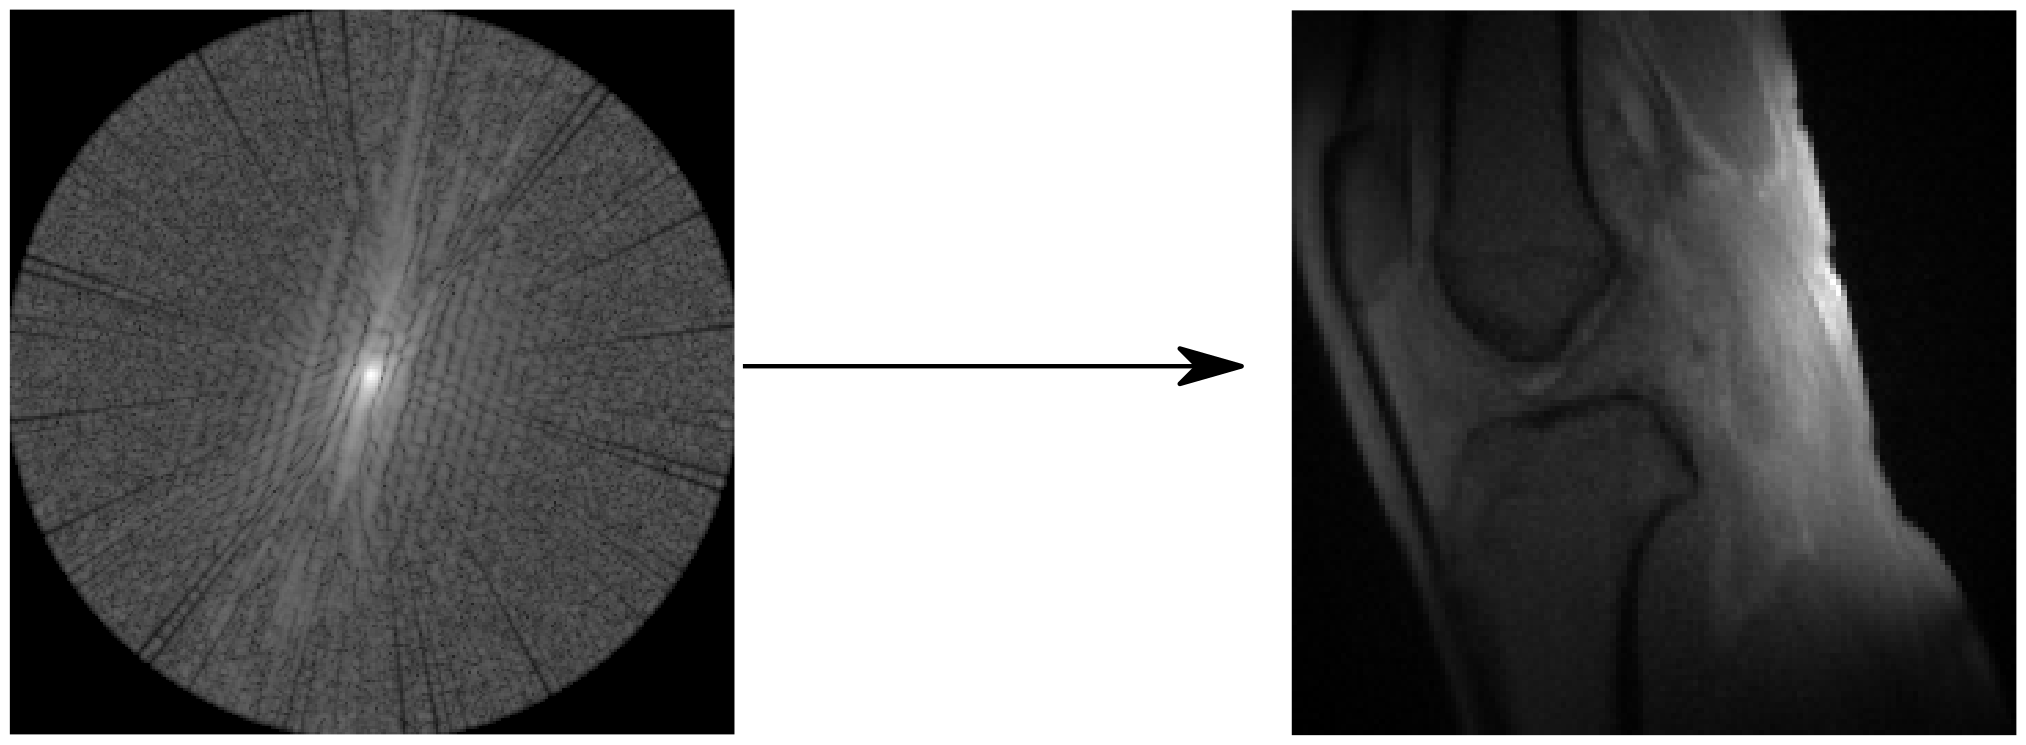
\includegraphics[width=0.9\linewidth, height=7.3cm]{kspace_arrow}
	\caption{\textbf{Example of k-space and reconstructed image}. Left: K-space data from a specific angle during the knee flexion cycle. Right: Corresponding reconstructed MRI image, illustrating the detailed visualization achievable through golden-angle sampling.}
	\label{fig:kspacearrow}
\end{figure}
  
\subsubsection{Gradient Echo FLASH sequence}

Gradient echo (GRE) imaging sequences are prime candidates for dynamic MRI because it is a fast scanning process. There are two major factors that contribute to its speed. First, unlike the spin echo, we do not need to wait for a long time for the longitudinal magnetization component $M_z$ to sufficiently recover for another repetition. This is because in a GRE sequence, a smaller flip angle can be used. Secondly, we do not need to wait for the spins to refocus after the application of a $180^o$ rf pulse, because there is no such pulse applied. Instead, the refocusing is done here by using magnetic field gradients of opposite polarity. The scheme of GRE sequence is depicted in Figure \ref{fig:gresimplified}. The notation is as follows: $\alpha^o$: flip angle (less than $90^o$), RF: radio frequency pulse, SS: slice selecting gradient, PE: phase encoding, FE: frequency encoding, TE: echo time and TR: repetition time. Note that in the frequency encoding direction, a negative dephasing lobe is followed by a positive gradient that brings the spins back into phase to generate the signal.    
\begin{figure}[H]
	\centering
	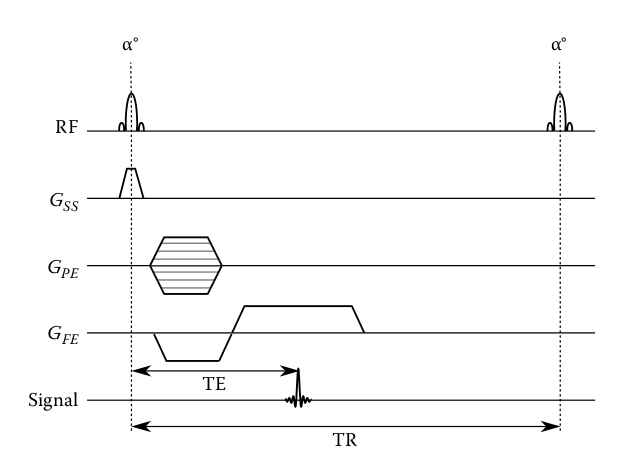
\includegraphics[width=0.7\linewidth]{gre_simplified}
	\caption{Simplified diagram of the GRE sequence that depicts the refocusing gradient applied in the frequency encoding direction \parencite[p.233]{berry_fundamentals_2009}.}
	\label{fig:gresimplified}
\end{figure}

After a series of rf pulses are applied, we reach a condition in gradient echo sequences called the \textbf{steady state.} In this state, the magnitude of the longitudinal magnetization component $M_z$ is the same at the end of every TR. Similarly, we can also have a residual transverse magnetization $M_{xy}$ at the start of every repetition cycle. If we deliberately dephase this residual transverse magnetization, the sequence is described as incoherent or spoiled gradient echo sequences.

FLASH is a type of spoiled GRE. It is a naming scheme that spells Fast Low-Angle Shot. \parencite{haase_flash_1986} The introduction of the FLASH technique in the 1980s, known for its rapid acquisition capabilities, marked a significant advancement in MRI technology. It allowed for clearer imaging of dynamic processes and reduced artifacts associated with movement. The original paper on FLASH highlights the technique's potential for "recording NMR movies" to visualize physiological changes, a capability now fully integrated into contemporary MRI practices.

\section{Methodology}
\label{sec:second}

\subsection{Data Collection Methods}

\subsubsection{Procedure Details}
Dynamic MRI scans were conducted on five healthy individuals, two females and three males, ranging in age from 28 to 39 years and weighing between 55 to 90 kilograms, utilizing a 3 T Siemens Prisma fit scanner. These volunteers were free from any known musculoskeletal disorders and provided their written consent, adhering to the ethical standards approved by the institutional review board. For all of these subjects, the left leg was scanned. In total, 7 unique datasets were acquired for analysis with two subjects measured twice on separate days to check for protocol stability. 


Once the subject was positioned supine in the scanner, the thigh was secured on a wedge positioner, and the lower leg was attached to an ankle rest, just above the malleoli, using Velcro straps to minimize lateral movement. The knee to be examined is aligned with the device’s axis of rotation, while the other leg rests alongside the MRI scanner's bore.  Knee motion is guided by a belt and sprocket assembly running alongside the lower leg, connected to a gearbox activated by the leg support as the participant flexes and extends the knee. Once the subject was positioned at the scanner's isocenter, their leg naturally assumed a flexed posture due to the design of the device. In this configuration, the leg is cradled by the device arm which is positioned below the level of the knee, ensuring that the leg remains flexed without the volunteer exerting any force.


The volunteer engaged in a controlled exercise, following a metronome set at 60 beats per minute. This pace dictates a four-beat flexion to extension cycle, with the leg being flexed at the first beat and fully extended by the fourth. This equals to 8 beats per cycle, or 7.5 cycles every minute. Initially conducted under a loaded condition with weights added to the distal end of the device, the process is repeated without the added resistance to compare both states. The scan duration is around two and a half minutes, amounting to 20 full flexion-extension-flexion cycles. The range of motion for each dataset is noted in table Blank. 

\begin{table}[H]
	\centering
	\label{tab:range_of_motion}
	\caption{Range of Motion for Different Datasets}
	\begin{tabular}{cc}
		\toprule
		Dataset & Range of Motion (°) \\
		\midrule
		1 & 30 \\
		2 & 38 \\
		3 & 36 \\
		4 & 30 \\
		5 & 36 \\
		6 & 36 \\
		7 & 46 \\
		\bottomrule
	\end{tabular}
	
	
\end{table}

\subsubsection{Sequence Parameters and Reconstruction}
Table \ref{tab:mri_seq_params}, lists the MRI sequence parameters along with their respective units.

\begin{table}[H]
	\centering
	\label{tab:mri_seq_params}
	\caption{MRI Sequence Parameters}
	\begin{tabular}{@{}ll@{}}
		\toprule
		Sequence Parameters & Values \\ \midrule
		Dimensions of raw data & (352, 276, 16, 100) \\
		Acquisition Duration & 160 [s] \\
		Dwell Time & 0.0024 [ms] \\
		Echo Time & 2.51 [ms] \\
		Field Strength & 2.89362 [T] \\
		Flip Angle & 8.0 [degrees] \\
		Field of View (FOV) & 192.0 x 192.0 x 3.0 [mm] \\
		Frequency & 123.25 [MHz] \\
		Inversion Time & 150000 [ms] \\
		Matrix Size & 176 x 176 x 1 \\
		Repetition Time & 5.8 [ms] \\
		\bottomrule
	\end{tabular}
\end{table}

In this study, the k-space data was acquired using 16 receive channels, each recording data simultaneously but with a unique spatial sensitivity profile. With 276 spokes used to sample a k-space dataset and a repetition time (TR) of 5.8 milliseconds per spoke, it takes approximately 1.6 seconds to acquire one k-space data. Over the course of the experiment, 100 such k-space datasets are acquired, equaling 100 repetitions as noted. The total scan duration extends just over two and a half minutes, a time frame reported by the subjects as being manageable, regardless of whether the scan was conducted under loaded or unloaded conditions.

Each k-space dataset contained data across a range of knee angles because of the continuous leg movement set to the metronome beat. This means, assuming the subjects perform perfectly in time of 60 beats per minute where we have 4 beats for flexion to extension, each k-space covers 0.4 times the range of motion. For example, a subject with a range of motion of $40^o$, each k-space dataset contains data across $16^o$. Therefore, with multiple repetitions, data across the full range of motion could be adequately acquired.      

\textbf{Reconstruction}


The MRI raw data, with dimensions of (352, 276, 16, 100), was processed using a reconstruction script to generate the final image dataset. These dimensions correspond to: 
\begin{itemize}
	\item 352: The number of data points per spoke.
	\item 276: The number of spokes used to sample a k-space dataset.
	\item 16: The number of receive channels
	\item 100: The number of repetitions or k-space datasets acquired over the course of the experiment.
\end{itemize}


First, the binary data from the optical sensor was loaded, and the physical angle information was grouped according to each repetition cycle. This was done by detecting significant changes in the trigger signal, which was obtained from the sensor data too. This grouping resulted in 100 groups, each containing the physical angle information for a specific repetition. For each repetition, spokes in k-space were assigned to their corresponding physical angles. An angle increment of 2 degrees was chosen, which led to a collection of spokes corresponding to each 2-degree range. This approach was applied to all repetitions, allowing spokes to be mapped to physical angles across the full range of motion.

Subsequently, reconstruction was performed on each group of spokes. Depending on the specific angle range, the number of spokes assigned varied between 300 and 1000. Additionally, the direction of leg movement—either from flexion to extension or vice versa—was determined by calculating the slope of the angle information. Images were then reconstructed separately for each direction, depending on whether the leg was moving upward or downward. This distinction is crucial because leg biomechanics vary significantly depending on whether the movement is working with or against gravity.

\textbf{The use of rielsing toolbox}

The actual image reconstruction was done by using the Riesling reconstruction toolbox \parencite{wood2020riesling}. This toolbox offers a range of advanced algorithms tailored for non-Cartesian MRI reconstruction. In this study, an Alternating Direction Method of Multipliers (ADMM) approach was employed, incorporating Total Generalized Variation (TGV) regularization. 

ADMM is an iterative optimization algorithm that breaks down complex problems into smaller subproblems to solve them efficiently. It ensures accurate reconstruction by maintaining a balance between the primal (actual solution) and dual (approximate solution) residuals. This balance is particularly important for non-Cartesian MRI reconstruction, given the unique geometry of the data. ADMM allows different regularization techniques, like TGV, to be applied simultaneously during reconstruction.\parencite{MAL-016} 

TGV is an advanced regularization method that reduces noise while promoting smoothness in the reconstructed images. Unlike basic Total Variation (TV) regularization, TGV allows for piecewise smooth transitions between different regions, making it better suited for images with varied structures. In this study, a regularization strength of 5e-2 was chosen empirically, striking a balance between noise suppression and edge detection.

The final reconstructed images were affected by the chosen reconstruction parameters, including the zero-filling factor and the field of view (FoV) trimming factor. The use of TGV regularization and the ADMM algorithm influenced the resulting image resolution, providing images with a consistent size suitable for downstream analysis. Each image frame was reconstructed with dimensions of (528, 528) and the number of frames were subject dependent. 


\subsection{Data Analysis}
All the analysis and data visualization were done using the python programming language (v3.11.5). Several distinct steps were performed to semi-automate the segmentation of tibia and femur. This involves first finding one boundary edge each for the bones, and then tracking them across the full flexion-extension cycle by computing their respective transformation matrices. 
 
\subsubsection{Segmentation}
The semi-auto segmentation process is achieved in five distinct steps as described below: 

\textbf{Step 1: Edge Detection}

The Canny filter \parencite{canny_computational_1986}, as implemented in the scikit-image's feature library (v0.21.0), was employed to apply an edge filter to the images. The Canny edge detection algorithm operates in several key steps to identify edges with high accuracy in images. Initially, the image is smoothed using a Gaussian filter to reduce noise and potential false edge detections. Following this, the algorithm calculates the gradient intensity and direction at each pixel, which helps in identifying the edges' boundaries.

Subsequently, the algorithm applies double thresholding, which involves two thresholds: a low and a high. This creates three categories of pixels: strong, weak, and non-edges. Pixels with intensities above the high threshold are marked as strong edge pixels, while those below the low threshold are considered to be non-edges. Pixels between these two thresholds are marked as weak edge pixels. Weak edge pixels are potentially converted into strong edges through a process known as hysteresis, where only those weak edges that are connected to strong edges are confirmed as true edges. In this context, hysteresis refers to the algorithm's reliance on the connectivity history of pixels to decide their edge status, ensuring that only meaningful, connected edges are preserved. This step is crucial for ensuring the continuity and completeness of detected edges.  

To optimize the edge detection specifically to capture the desired edges of the tibia and femur, the different parameters like the standard deviation of gaussian blur (sigma) and the thresholds were tested in different combinations. The optimal results were achieved with a low threshold between 0 to 5 and a high threshold between 6 to 10. The sigma value was set at 2. Figure \ref{fig:edgemitimg} displays the output of with these parameters.  
\begin{figure}[H]
	\centering
	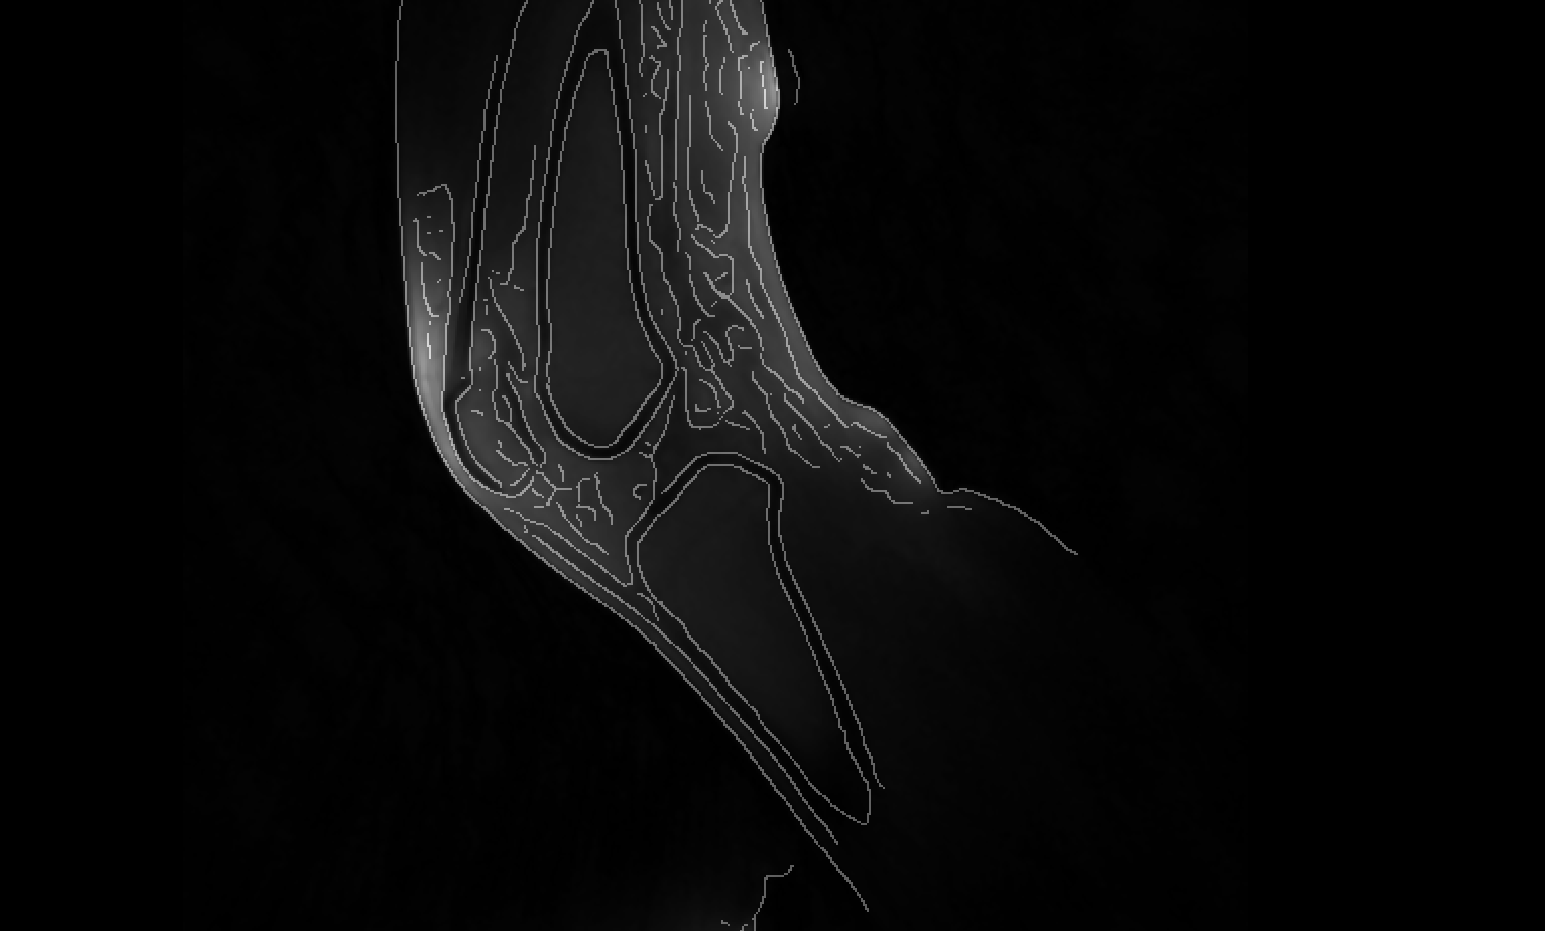
\includegraphics[width=0.7\linewidth]{edge_new}
	\caption{Output of the Canny edge detection algorithm applied to one of the frames, showing the detected edges of the tibia and femur bones overlayed on top of the original image for visual comparision.}
	\label{fig:edgemitimg}
\end{figure}


Subsequently, the scikit-image's morphology library was utilized to remove small elements from the binary image. The image was then skeletonized to a one-pixel width, retaining only long and consistent edges. It should be pointed out that the final edge does not necesarrily need to span the full boundary of the interior edge of the cortical bone; even partial edges were successfully used for this purpose.  

\textbf{Step 2: Labelling}

For the final selection of the desired edges, a labeling algorithm (`ndimage.label`) from SciPy, an open-source Python library designed for scientific computing (version 1.11.3), was utilized. The purpose of employing this labeling algorithm is to effectively isolate specific structural features, such as distinguishing the interior cortical bone from the exterior, by assigning unique labels to separate closely situated edges detected in the image. This algorithm applies the principle of connected-component labeling,  a method used in computer vision to detect connected regions in binary digital images. Connected-component labeling algorithm scans an image and groups its pixels into components based on pixel connectivity, meaning that all pixels in a connected component share similar pixel values and are adjacent to each other.

The labeling process treats any non-zero values in the input array as part of potential edges and zero values as background. The connectivity of these components is determined by a structuring element, which in this case was a fully connected 3x3 matrix:
$$
\begin{bmatrix}
	1 & 1 & 1 \\
	1 & 1 & 1 \\
	1 & 1 & 1
\end{bmatrix}
$$
This matrix is crucial as it defines the connectivity rules used during the labeling. Each pixel is considered connected to its eight immediate neighbors (above, below, left, right, and diagonals), known as eight-way connectivity. This element was chosen by trial and error. Alternatives, such as a four-way connectivity matrix, were tested but gave different labels to the same edge across frames. By using the eight-way connectivity, the same edge maintains consistent labeling across all frames, simplifying the analysis and reducing the need for manual adjustments. 

Figure \ref{fig:labelimg} shows the output from the labelling algorithm, where each color represents a separate label. 

\begin{figure}[H]
	\centering
	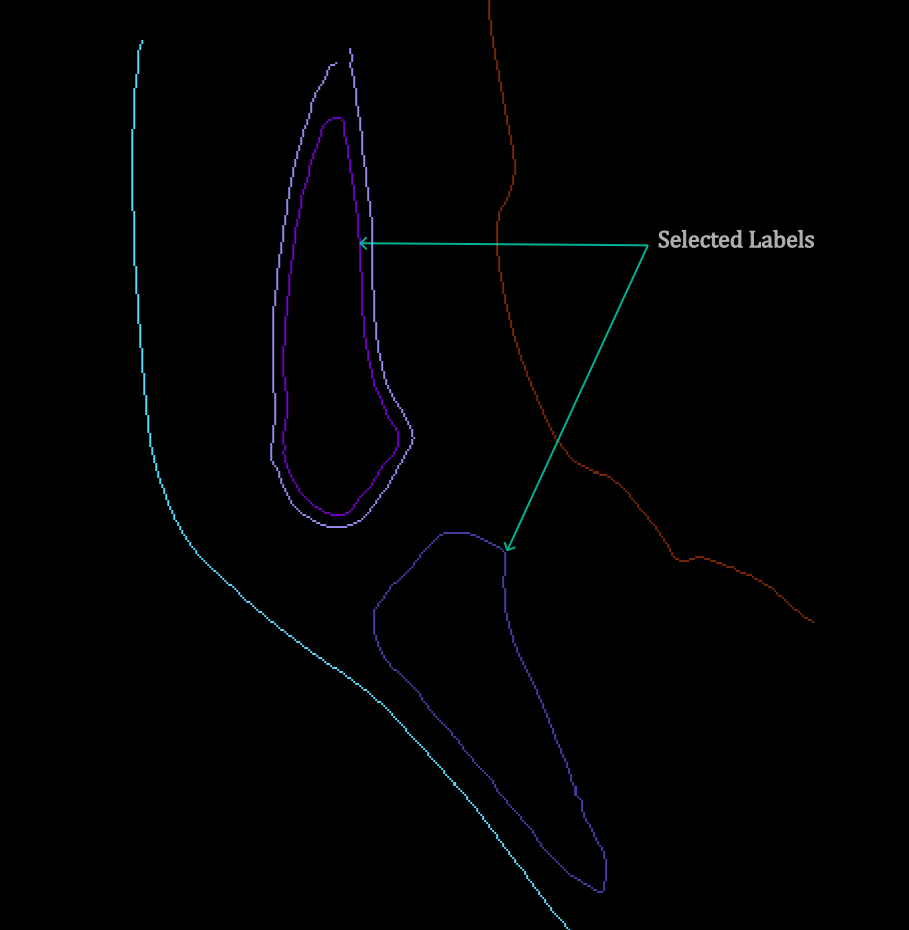
\includegraphics[width=0.7\linewidth]{label_selected}
	\caption{Output from the labeling algorithm with the representative edges for femur (top) and tibia(bottom) pointed out.}
	\label{fig:labelimg}
\end{figure}
 
After choosing the appropriate labels, a binary image for each frame is obtained, where the foreground has the boundary for the interior edge of tibia and femur, and the background has intensity value of zero.   

\textbf{Step 3: Obtaining the set of reference points}

Upon successfully isolating the binary edge images of the tibia and femur in Step 2, the subsequent step deals with establishing a set of reference points along each bone's edge in the first frame. This frame, captured when the knee is in a fully flexed position, serves as the reference frame for further analysis.  This frame is chosen as the baseline (where transformations are initialized to zero) to facilitate the accurate calculation of rotation and translation matrices that describe the movement of the knee through subsequent frames. The purpose of establishing these reference points is twofold: to simplify the complex data set for efficient processing and to ensure a consistent basis for accurately calculating transformations between subsequent frames. This is essential, as direct use of the densely packed binary edge data would be computationally cumbersome and less precise for such transformations.

To begin, the points along the boundary were organised and sorted. This was done by first, defining a starting point, and then iteratively using a greedy nearest neighbor algorithm for sorting. The most distal point of the bone was taken as the initial seed. Various functions from the numeric python library 'Numpy' (v. 1.26.4) were employed for this task. 


Once the points are sorted, the next step involves downsampling these points to a set of uniform equidistant reference points along the boundary of the binary edge. The necessity for this step arises from the inherent irregularity and density of the binary edge data. Directly sampling every n-th point from the sorted list would not suffice, as it could result in uneven spacing due to the variable distances between consecutive points in the original data.

This process begins by calculating the cumulative distances between each consecutive pair of points in the sorted list. Using these distances, a total path length is established. The desired interval between the new points is then determined by dividing this total path length by the number of intervals (number of desired points minus one). 

Determining the optimal number of points—ranging between 50 to 80—was established through trial and error. Fewer than 50 points often compromised the accuracy of the edge overlap by failing to capture the essential contours of the bone. Conversely, exceeding 80 points did not significantly enhance the algorithm's accuracy but increased the code execution time slightly. 

To achieve precise positioning of these points, cubic spline interpolation from SciPy's interpolate libary was used. This interpolation method is particularly effective for ensuring that the new points adhere closely to the original curve while maintaining equidistance. 
Figure \ref{fig:downsampled} depicts this result. 
\begin{figure}[H]
	\centering
	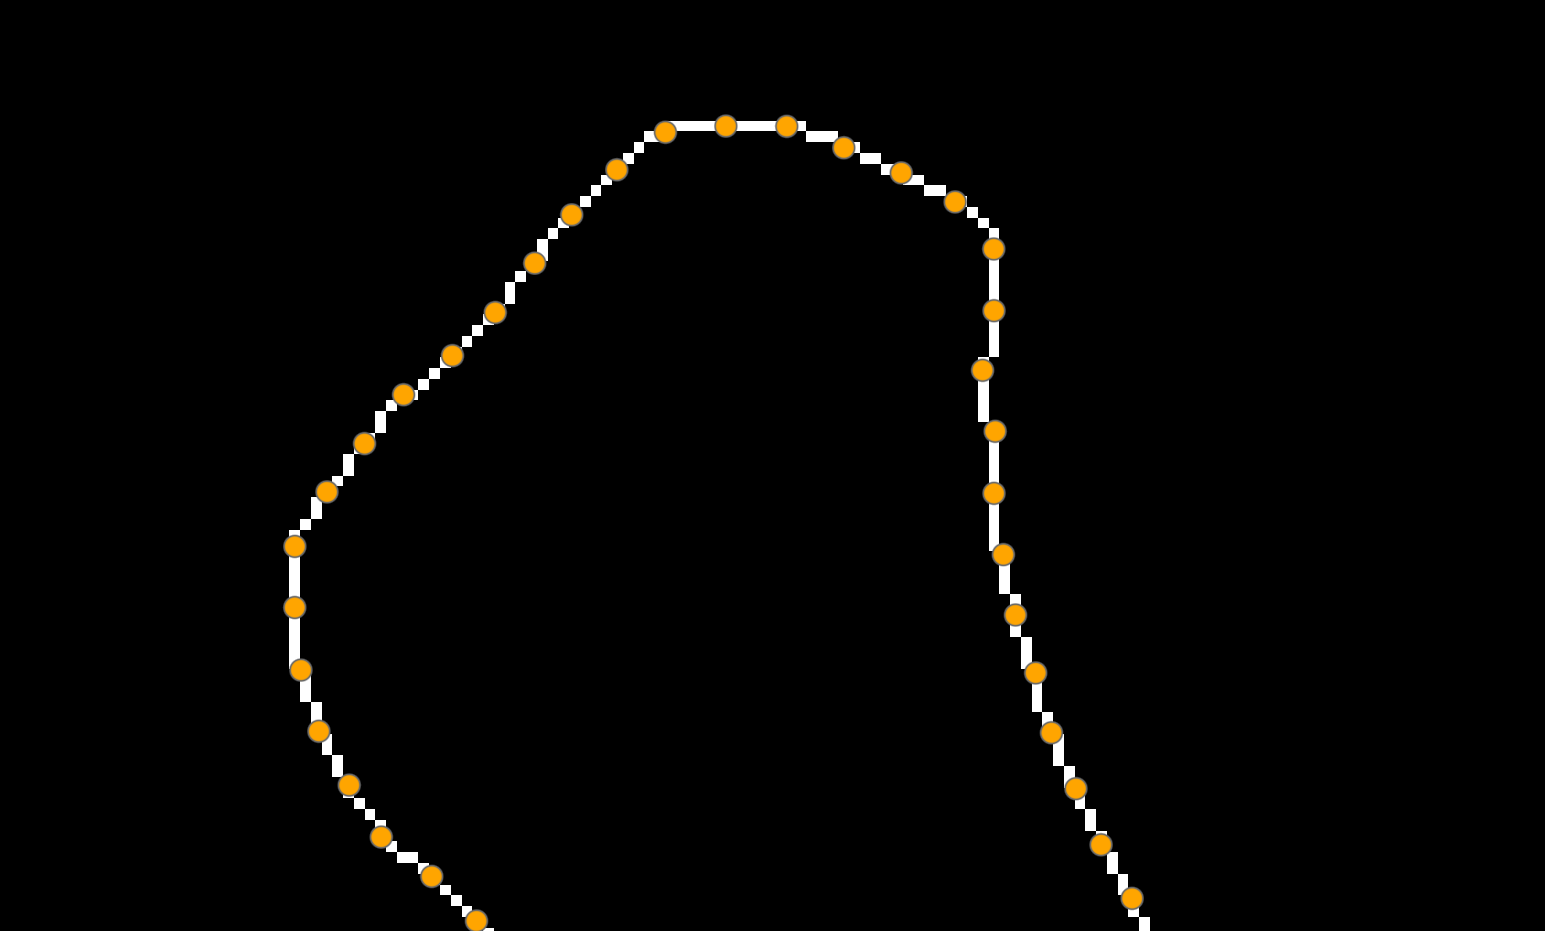
\includegraphics[width=0.7\linewidth]{downsampled}
	\caption{A zoomed in look at the equidistant sampled points (orange) along the boundary of the tibia edge (white).}
	\label{fig:downsampled}
\end{figure}

\textbf{Step 4: Transformation matrices computation}

In this step, a set of transformation matrices is obtained, each containing the parameters that align a segment of the bone from one frame to the next. These transformations includes solely the translation in the sagittal plane and rotation about the transverse axis. This approach assumes that the bone does not undergo any deformation and that through-plane motion is negligible throughout the motion cycle. 

Mathematically, the transformation of each point from one frame to the next can be expressed as 
\begin{equation}
	p^{'} = R(\phi)p + t
	\label{eq:rot} 
\end{equation}
where: 
\begin{itemize}
	\item \textbf{$p$} is the coordinate of the point in its current frame
	\item \textbf{$p^{'}$} is the coordinate of the point after transformation
	\item $\phi$ is the angle of rotation
	\item \textbf{$R(\phi)$}  is the rotation matrix, given by 
	 \[
	 R(\phi) = 
	 \begin{bmatrix}
	 	\cos \phi & -\sin \phi \\
	 	\sin \phi & \cos \phi
	 \end{bmatrix}
	 \]
	 
	 \item $t$ is the translation vector,
	 	\[
	 	t = \begin{bmatrix}
	 		x \\
	 		y
	 	\end{bmatrix}
	 	\]
 	\item x and y are the translations in the Cartesian coordinate system. 
\end{itemize}   
As such, only three parameters, $x$, $y$, and $\phi$ need to be computed. To determine these parameters, a cost function is defined. This function, denoted as $C(x,y,\phi)$, quantifies the alignment error by calculating the 'cost' of deviations for any given set of transformation parameters. The minimization of this cost identifies the combination of parameters that achieves the best alignment or overlap of the transformed frame with the reference frame. A lower value of the cost function output indicates a closer match to the target frame, suggesting a superior alignment, whereas a higher value signifies a less accurate alignment. The cost function is defined in Equation \ref{eq:cost_func}:  
\begin{equation}
	C(x, y, \phi) = \sum_{p=1}^{N} \min_{q \in Q} \left( \sqrt{(x_q - x_p')^2 + (y_q - y_p')^2} \right)
	\label{eq:cost_func}
\end{equation}
where:
\begin{itemize}
	\item $ (x_p, y_p) $ are the coordinates of points in the reference frame
	\item $(x_p', y_p')$ are the coordinates of points after transformation:
	\begin{align*}
		x_p' &= x + x_p \cos(\phi) - y_p \sin(\phi) \\
		y_p' &= y + x_p \sin(\phi) + y_p \cos(\phi)
	\end{align*}
	\item $(x_q, y_q)$ are the coordinates of points in the target frame.
	\item $N$ is the number of points in the reference frame, and $Q$ represents all points in the target frame.
\end{itemize}

This cost function evaluates the alignment of transformed coordinates to target coordinates by calculating the sum of the shortest distances from each point in the transformed frame to the closest point in the target frame. Each $(x_p', y_p')$ is the position of a point from the reference frame after being transformed by the parameters $x$, $y$, and $\phi$. For each transformed point,the distance to every point $(x_q, y_q)$ in the target frame is computed, the minimum of these distances is selected, and sum these minimum distances across all points is calculated. This sum forms the output of the cost function, which we seek to minimize.

The optimization of this cost function is performed using a nonlinear least squares approach. where the initial guess of [0,0,0] is provided. This guess represents the starting point for the transformation parameters $x$, $y$ and $\phi$. The \texttt{fmin} function from SciPy’s optimization module is used for this purpose, which uses the Nelder-Mead simplex method \parencite{nelder_simplex_1965}.   The function is configured with a function tolerance and parameter tolerance of $1 \times 10^{-8}$, and maximum iterations of 1000. This method iteratively explores the parameter space to find the set of parameters that result in the lowest cost function value. The optimization procedure continues until the change in the cost function is less than the specified tolerance or the maximum number of iterations is reached, indicating convergence to an optimal solution. Figure \ref{fig:edge_tracking} provides a visual representation of the overlap of the reference points from the fully flexed initial position to the frame where the lower leg has been rotated by an angle of 12 degrees as reported by the rotary angle encoder. 
\begin{figure}[H]
	\centering
	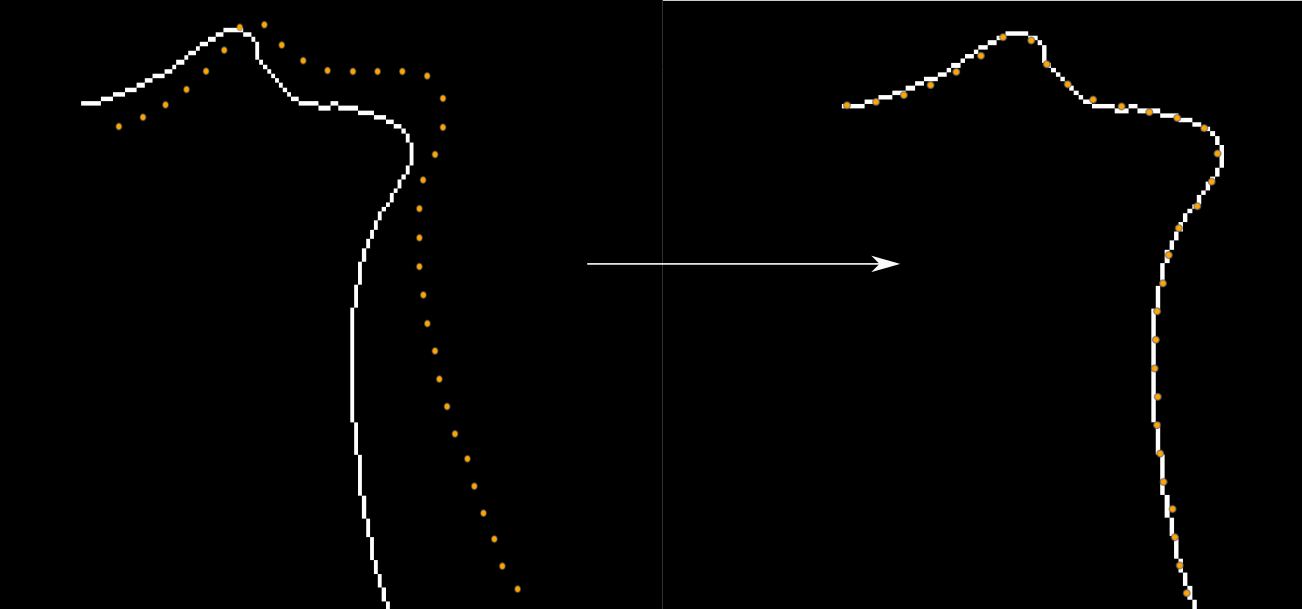
\includegraphics[width=0.7\linewidth]{image137}
	\caption{Left: The reference points in the first frame (orange) overlaid with the binary edge image of the target frame (white).Right: The reference points have been transformed by using the results from the optimization showing almost perfect overlap, illustrating the effective alignment achieved through the minimization of the cost function.}
	\label{fig:edge_tracking}
\end{figure}

\textbf{Step 5: Auto-Segmentation }

With the transformation matrices obtained for the femur and the tibia, manual segmentation is performed on the first frame. An example is given in figure \ref{fig:manualsegment}. 
\begin{figure} [H]
	\centering
	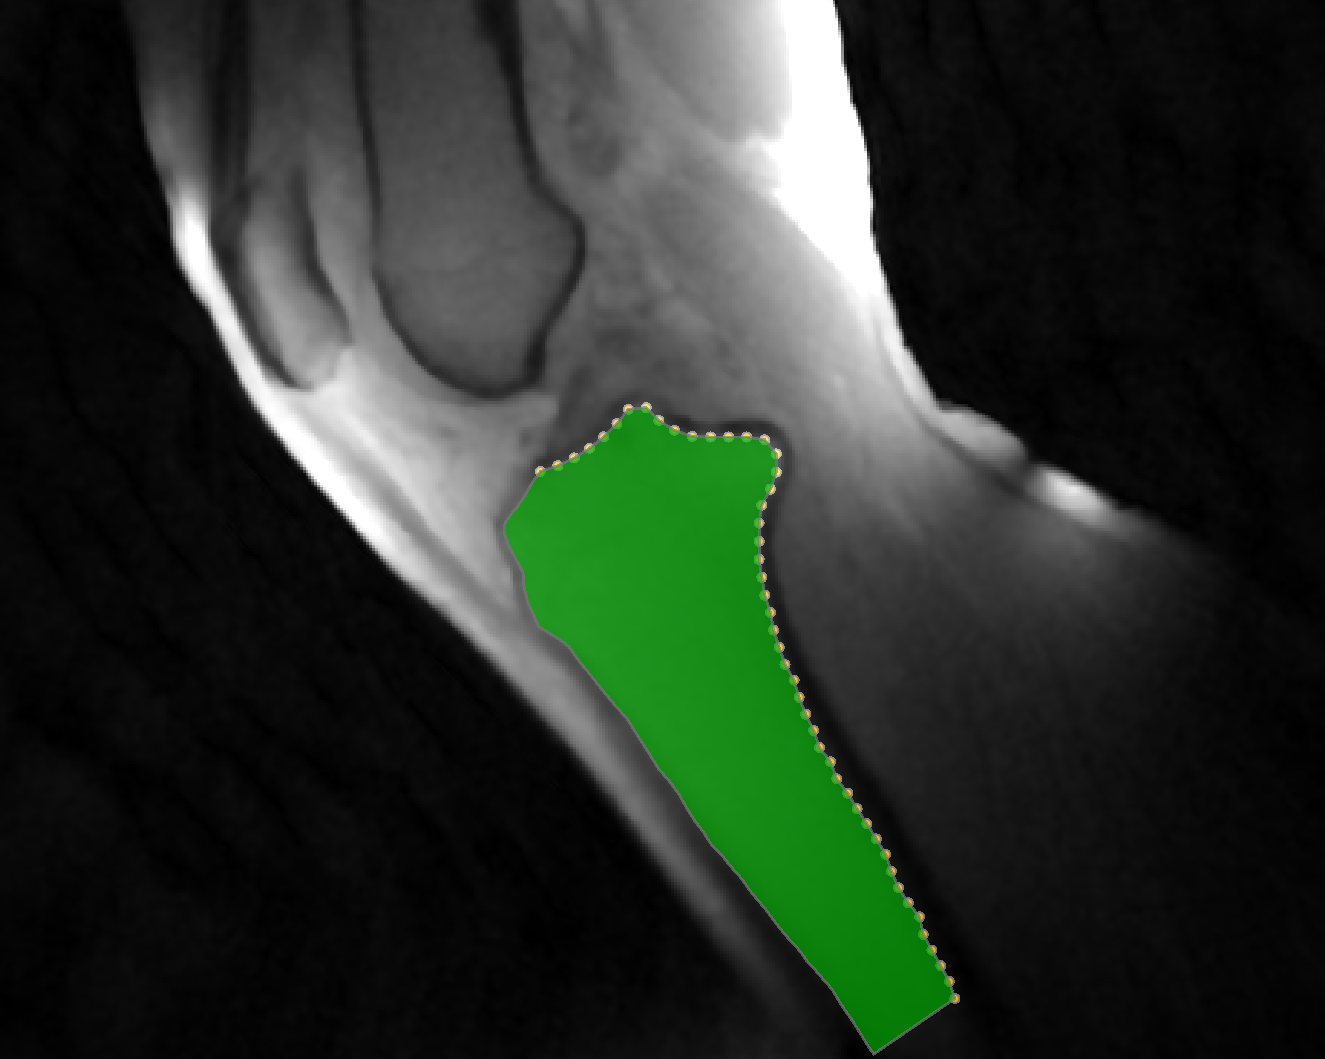
\includegraphics[width=0.7\linewidth]{manual_segment}
	\caption{Manual segmentation is performed to complete the boundary of the tibia's interior edge shown in green, along with the reference points (orange).}
	\label{fig:manualsegment}
\end{figure}

Using the points from this segment, the transformation matrices are now applied once more using equation \ref{eq:rot} to transform one frame to the next subsequently to complete the full segmentation across all the frames automatically. 

\subsubsection{Extraction of Biomechanical Parameters}
After achieving automated segmentation of the tibia and femur across all frames, the next step involved extracting biomechanical parameters from the segmented regions. Two key metrics were considered for analysis to assess the relationship between these bones throughout the flexion-extension cycle captured in the 2D Cine images.

The first metric involved calculating the angle between the long axis of femur and tibia segments. This measurement provided insight into how the relative orientation of the two bones changes over time.

The second metric measured the distance between specific anatomical landmarks on both the femur and tibia. Tracking this distance across the frames offered an understanding of how the spatial relationship between these two bones evolved during the motion cycle. 

\textbf{Angle between the bones}

To calculate the angle between the bones, the long axis of each bone segment was identified using a technique called Principal Component Analysis (PCA). The analysis was performed using the PCA implementation from the scikit-learn (v1.3.1) Python library, a module for machine learning built on top of SciPy.

PCA determines the direction of maximum variance in the data, which coincides with the longitudinal axis of the bone. PCA first uses the coordinates of the segmented binary mask as input. The centroid of the shape is calculated and subtracted from each data point, centering the data such that the mean of this transformed data is (0, 0). 

Next, the covariance matrix (\text{Cov}) is computed, a square matrix that gives an indication of how the data varies along each dimension and how different dimensions vary together. 

\begin{equation}
	\text{Cov} = 
	\begin{bmatrix}
		\mathrm{Var}(X) & \mathrm{Cov}(X,Y) \\
		\mathrm{Cov}(Y,X) & \mathrm{Var}(Y) \\
	\end{bmatrix}
	\label{eq:cov}
\end{equation}

where:
\begin{itemize}
	\item \(\mathrm{Var}(X)\) is the variance of \(X\), given by:
	\[
	\mathrm{Var}(X) = \frac{1}{N-1} \sum_{k=1}^{N} (X_{k} - \bar{X})^2,
	\]
	where \(N\) is the number of points, \(X_{k}\) represents the \(k^{th}\) observation in the \(X\) dimension, and \(\bar{X}\) is the mean value of all observations in the \(X\) dimension. 
	\item \(\mathrm{Cov}(X,Y)\) is the covariance between dimensions \(X\) and \(Y\), defined as:
	\[
	\mathrm{Cov}(X,Y) = \frac{1}{N-1} \sum_{k=1}^{N} (X_{k} - \bar{X})(Y_{k} - \bar{Y}),
	\]
	where \(Y_{k}\) represents the \(k^{th}\) observation in the \(Y\) dimension, and \(\bar{Y}\) is the mean value of all observations in the \(Y\) dimension.
	
	\item \(\mathrm{Cov}(Y,X)\) is equivalent to \(\mathrm{Cov}(X,Y)\) because the covariance matrix is symmetric.
	
	\item \(\mathrm{Var}(Y)\) is the variance of \(Y\), calculated similarly to \(\mathrm{Var}(X)\).
\end{itemize}

When this covariance matrix is applied to a vector, the matrix transforms the vector such that it aligns more closely with the direction of maximum variance in the dataset. Therefore, by computing the matrix's eigenvectors and eigenvalues, the vectors representing the direction of maximum variance is identified. The first principal component refers to the eigenvector associated with the largest eigenvalue. In figure \ref{fig:longaxes}, the longitudinal axis of femur and tibia are shown. 

\begin{figure}[H]
	\centering
	\includegraphics[width=0.7\linewidth]{theta_angle}
	\caption{The long axis of the bones are identified by using the PCA (blue) along with the centroid (white cross) for each segment. $\theta$ represents the angle that is being measured}
	\label{fig:longaxes}
\end{figure}

The angles between the segments was calculated by using the dot product between unit vectors, as given in equation \ref{eq:angle}

\begin{equation}
	\theta = \arccos(\mathbf{U}_{fem} \cdot \mathbf{U}_{tib})
	\label{eq:angle}
\end{equation}
where, $\mathbf{U_{fem}}$ and $\mathbf{U_{tib}}$ are the unit vectors of the longitudinal axes for the femur and tibia segments respectively. For visualization purposes, when the knee is hyperextended, angles greater than 180° are reported to clearly indicate the degree of hyperextension. Therefore, in graphs presenting the results, the peak angle can exceed 180° (e.g., 185°) to represent hyperextension. 

\textbf{Distance between the bones}

To calculate a proxy for the distance between the bones, anatomical landmarks were identified for the bones. The most distal point on the femur segment was chosen for the femur and a point on the proximal tibia for the tibia as shown in figure \ref{fig:twopoints}.   
\begin{figure}[H]
	\centering
	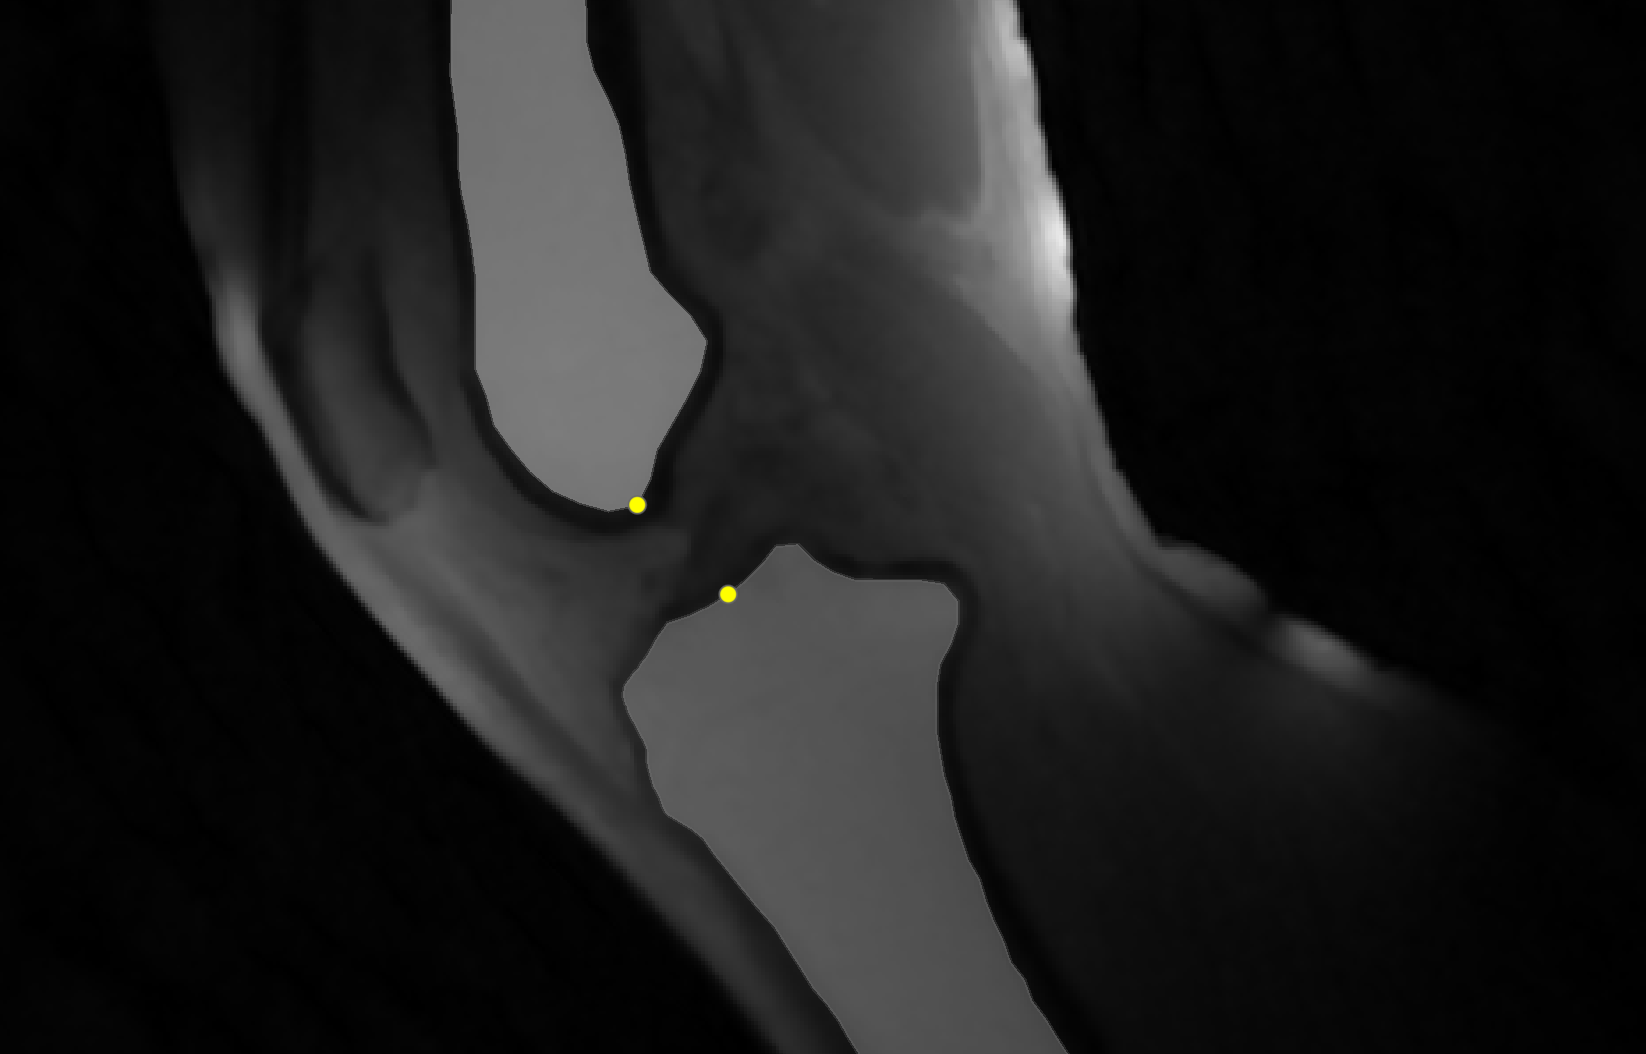
\includegraphics[width=0.7\linewidth]{two_points}
	\caption{Points based on anatomical landmarks are shown in yellow.}
	\label{fig:twopoints}
\end{figure}

The euclidean distance between these two points was measured across time by using equation \ref{eq:distance}. The first frame at -100\% flexion is considered as the baseline, with the distance set to 0 mm. All subsequent distances are relative to this baseline, enabling an analysis of changes across the cycle. 
\begin{equation}
	d = \sqrt{(y_2 - y_1)^2 + (x_2 - x_1)^2}
	\label{eq:distance}
\end{equation} 

Negative values imply the distance has decreased with respect to the baseline (first frame). 

\section{Results}
\label{sec:yetanother}

\subsection{Edge tracking and segmentation}

To evaluate the accuracy of edge tracking achieved through cost function minimization, the deviation of overlap between points on the transformed frame and the target frame was measured. The cost function output, which indicates the overlap accuracy, calculates the minimum distance from each point on the transformed frame to the points on the target frame and sums these minimum distances for all points in the transformed frame.

The mean alignment error per point was then derived by dividing the cost function output by the total number of points in the transformed frame. This value quantifies the average distance that a point on the transformed frame deviates from its corresponding point on the target frame. This value was calculated for all frames, and the average of these values was taken for each dataset.

The bar chart in Figure \ref{fig:avgofavg} presents this result: 

\begin{figure}[H]
	\centering
	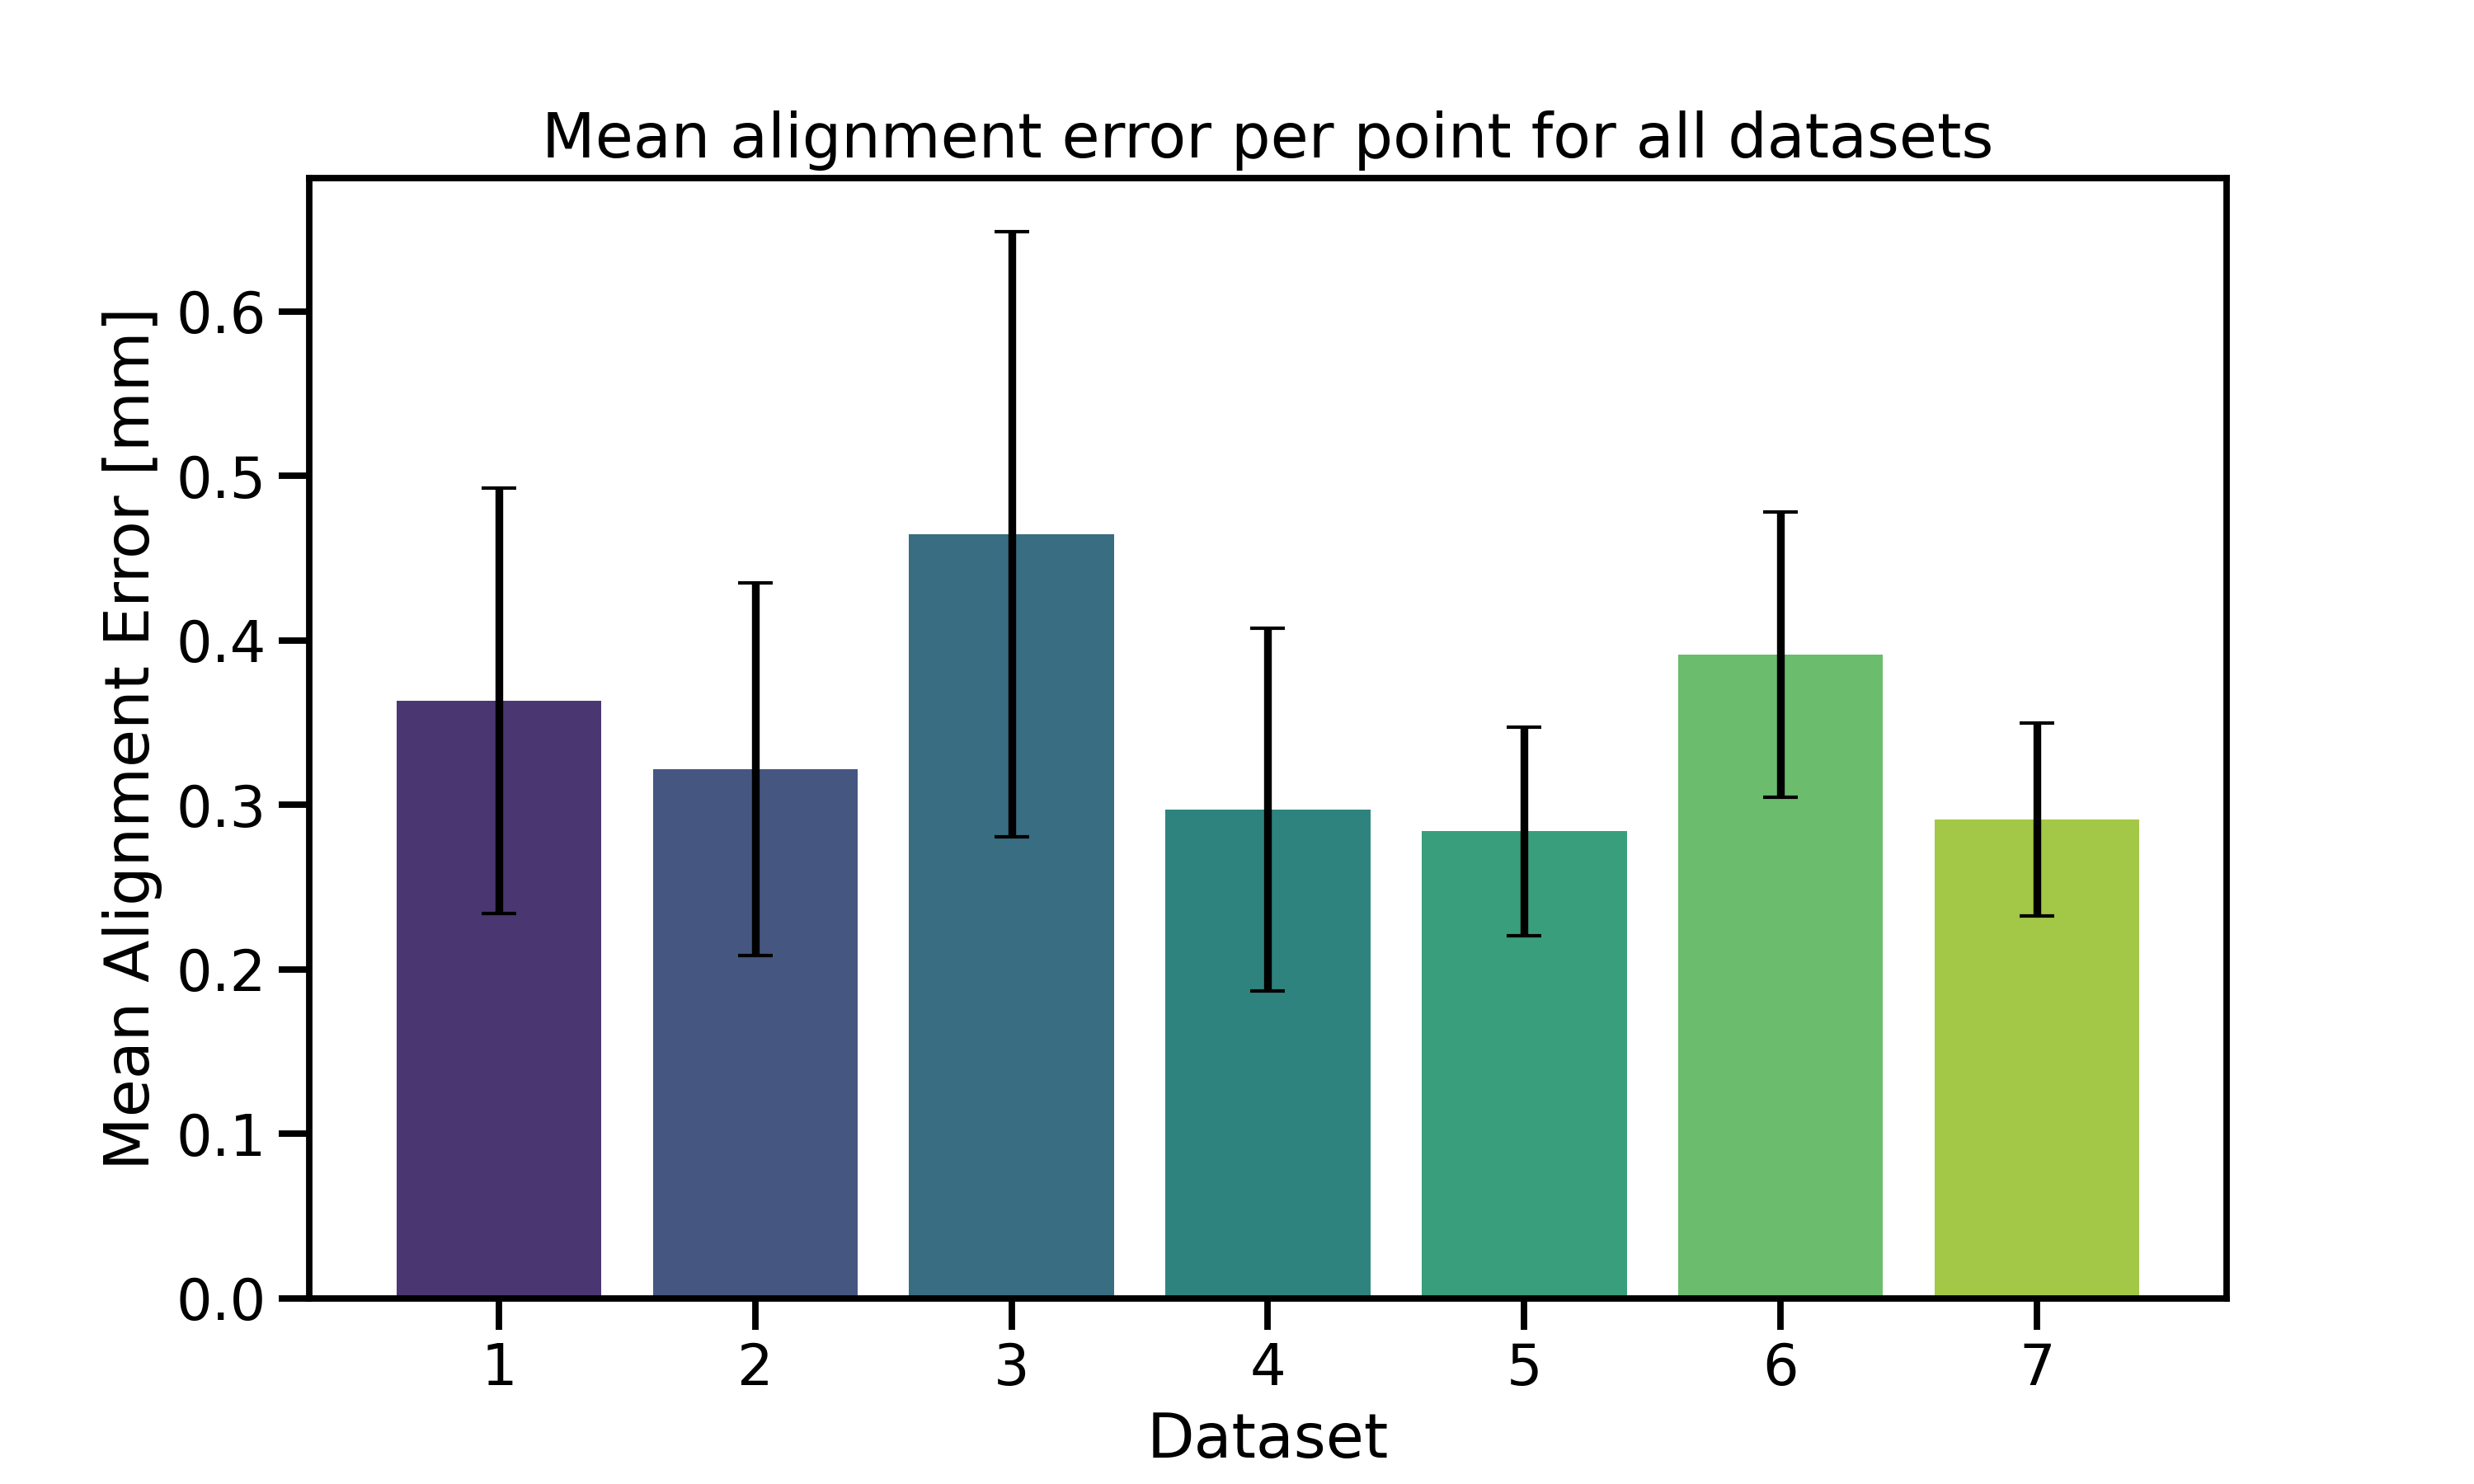
\includegraphics[width=0.7\linewidth]{bar_alignment}
	\caption{Mean alignment error per point across all frames for each tibia dataset.}
	\label{fig:avgofavg}
\end{figure}


The result of the segmentation for one of the datasets is given in figure \ref{fig:fullsegmented}. 

\begin{figure}[H]
	\centering
	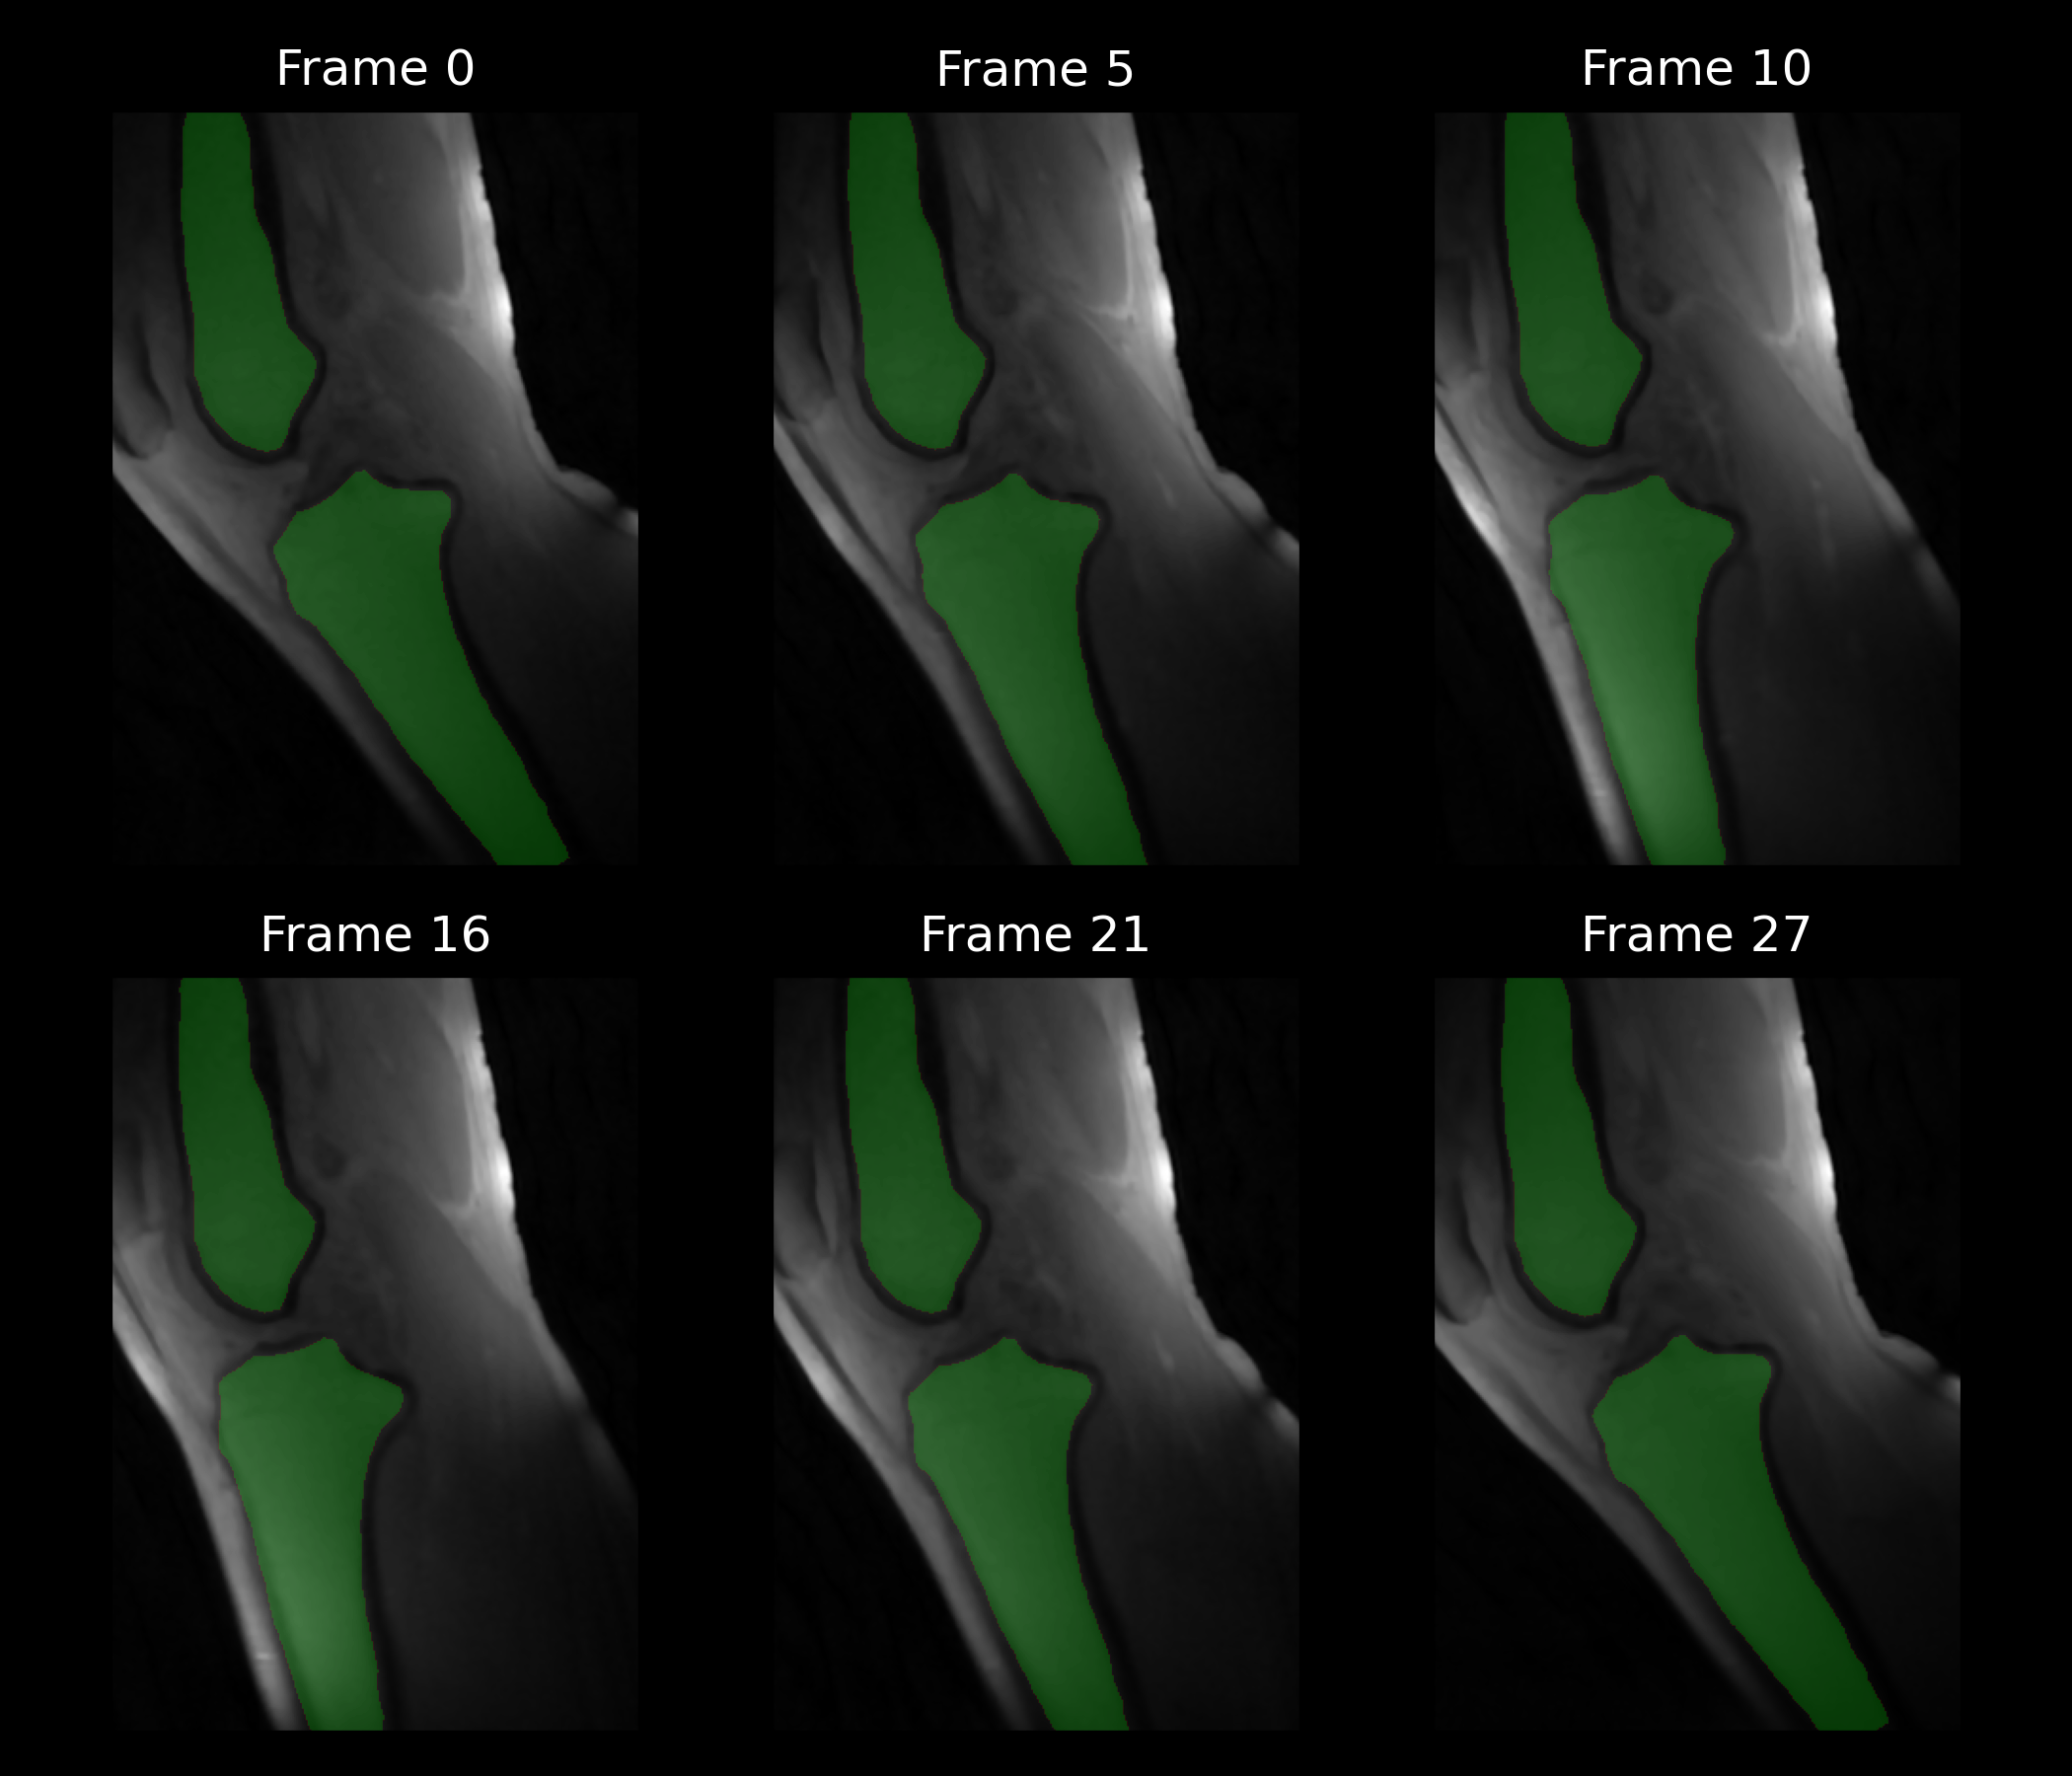
\includegraphics[width=0.7\linewidth]{full_segmented}
	\caption{A mosaic showing the segmented tibia and femur shapes(green) where each tile is a particular time point. The leg is fully flexed at Frame 0}
	\label{fig:fullsegmented}
\end{figure}

\subsection{Biomechanical parameter extraction}
The changes in the angle between the long axes of the tibia and femur segments, as well as the distance between these segments, were measured throughout the flexion-extension cycle for both the loaded and unloaded conditions.

To enable consistent comparisons across different datasets, the number of frames from each motion cycle was normalized by grouping the data into 'bins'. This binning process ensured that all datasets spanned the same range, allowing for the averaging and plotting of values within these bins.

The x-axis of the graphs represents the percentage of the flexion-extension cycle, defined by the bin centers. The cycle starts at -100 \% (maximal flexion), progresses to 0 \% (full extension), and returns to 100 \% (maximal flexion). This labeling captures the complete motion cycle, from full flexion to full extension and back to full flexion, allowing a clear visualization of the entire range of motion. The x-axis ticks correspond to the centers of these bins, with each bin having a width of 10 percentage units. 

The y-axis of the graphs represents the average value of the biomechanical parameter (either angle or distance) within each bin, aggregated across all datasets. 

For statistical analysis, a two-sample independent t-test was performed using the \texttt{stats} module from the  SciPy library to compare the loaded and unloaded conditions. The test was applied to the data within each bin to determine if there were significant differences between the two conditions.

\textbf{Angle calculation}

Figure \ref{fig:anglegraphstickman} displays the result of calculating the angle between the long axes of bone segments across the flexion-extension cycle. 
 
\begin{figure}[H]
	\centering
	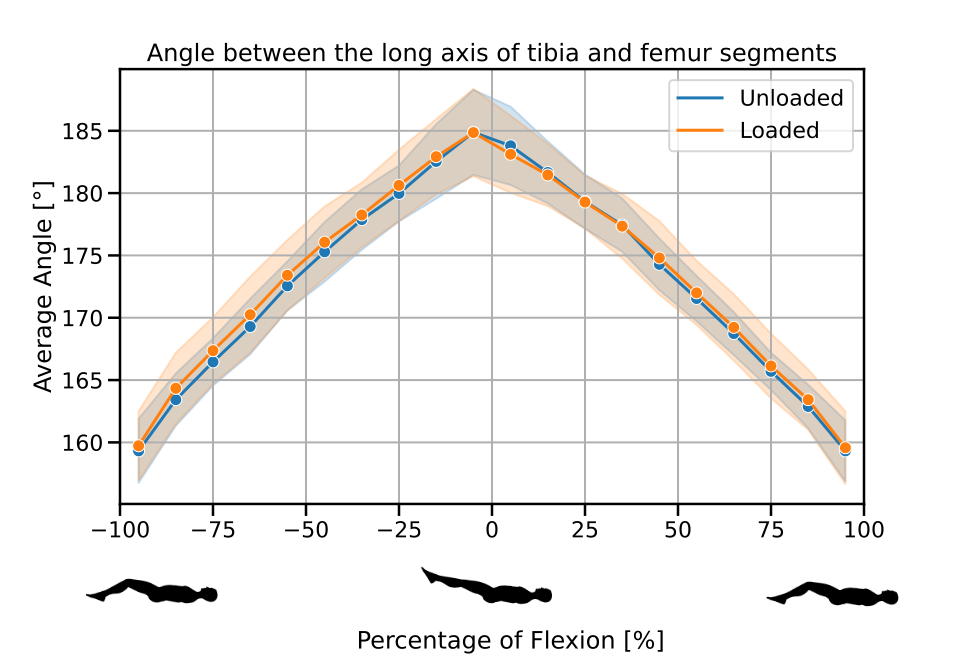
\includegraphics[width=0.7\linewidth]{angle_graph_stickman_modified}
	\caption{Plot of angle between long axes of bone segments between tibia and femur versus the flexion percentage.The x-axis ticks represent the centers of bins, each with a width of 10 percentage units. The shaded regions represent one standard deviation uncertainty. Angles greater than 180° imply hyperextension.}
	\label{fig:anglegraphstickman}
\end{figure}

No significant differences were observed between the loaded and unloaded conditions for any of the bins.

\textbf{Distance calculation }

The Euclidean distance between two points on the tibia and femur segments was measured throughout the flexion-extension cycle for both loaded and unloaded conditions. The aggregated results are shown in Figure \ref{fig:resultsdistancestickman}
\begin{figure}[H]
	\centering
	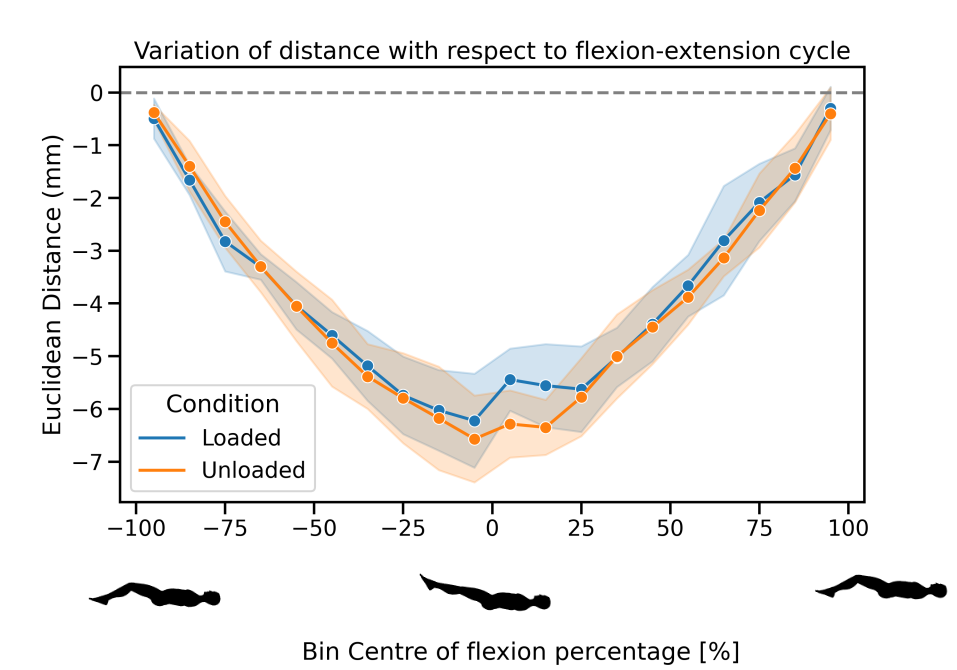
\includegraphics[width=0.7\linewidth]{results_distance_stickman}
	\caption{Plot showing the variation of euclidean distance between two points with across time in the motion cycle. All distances are relative to the baseline measurement at -100\% flexion, set at 0 mm. The shaded region represents one standard deviation uncertainty.}
	\label{fig:resultsdistancestickman}
\end{figure}

Statistical analysis revealed significant differences between loaded and unloaded conditions in the following bins: (0.0, 10.0] with a P-value of 0.022, and (10.0, 20.0] with a P-value of 0.015. No significant differences were observed for the remaining bins.

\section{Discussion}

The accuracy and reliability of the measurements obtained from the dynamic MRI scans are influenced by several factors that need to be considered to ensure meaningful results. One significant factor is the overall bulk movement of the leg during the scan. If the femur is not properly fixated, the entire leg might shift, leading to inaccurate measurements. Ensuring that the thigh is securely positioned on the device with the thigh strap is critical for minimizing this movement. Additionally, improper fixation can allow the upper leg to lift or shift laterally, further compromising the accuracy of the measurements. This overall instability can be exacerbated by the entire leg shifting longitudinally within the scanner, causing misalignment and poor-quality output.

Another important factor is muscle exhaustion. At the start of the exercise, volunteers might overexert themselves, leading to fatigue as the exercise progresses. This can cause variations in the range of motion and affect the position of the leg, resulting in inconsistent data. While the controlled exercise pace, guided by a metronome, aims to standardize the movement, individual differences in endurance can still introduce variability.

By addressing these factors, we can enhance the reliability of the measurements obtained from the dynamic MRI scans. With these considerations in mind, the following sections discuss the specific results of edge tracking and segmentation, angle measurement, and distance calculation in detail.

\subsection{Edge tracking and segmentation}
The accuracy of segmentation in this study is fundamentally tied to the precision of edge tracking, as the segment boundary is defined by the detected edges. A significant factor that compromises edge tracking accuracy is the through-plane motion of the bones, leading to inaccurate transformations. The algorithm is specifically designed to manage only rigid transformations within a single plane; therefore, any deviations introduced by through-plane motion significantly impair edge detection and, consequently, segmentation accuracy.

Through-plane motion is particularly problematic for the tibia compared to the femur, primarily due to medial/lateral rotation as illustrated in Figure \ref{fig:sixdegrees}, which details the six degrees of freedom of the tibia's movement relative to the femur. This specific type of rotation is a significant cause of through-plane motion errors during edge tracking, as the device setup—although restrictive—allows some degree of rotational freedom. Despite the lower leg being secured at the ankle with Velcro straps and the knee cradled in a wedge positioner to limit movement predominantly to one plane, complete immobilization is not achievable. This limitation is especially pronounced in subjects with smaller bones, where even additional padding at the wedge positioner was insufficient to prevent all undesired motion. While localizers are employed prior to the scans in both extended and flexed positions to ensure that the slice moves only within a predetermined single plane, certain rotations cannot be fully corrected by simply angling the localizer and may still be evident in the final images.

The performance of the edge tracking algorithm is illustrated by the bar chart in Figure \ref{fig:avgofavg}, which shows the mean alignment error per point across seven different datasets in millimeters. Datasets 2,4,5 and 7 show the lowest mean alignment error around 0.3 mm, with Dataset 5 having the lowest error of 0.283 mm and standard deviation of 0.063 mm. In contrast, Dataset 3 exhibits the highest mean alignment error at about 0.465 mm and also shows the largest variability with a standard deviation of 0.184 mm. This variability and higher error could suggest specific challenges in edge detection for this dataset, potentially due to factors such as through-plane motion or variations in image quality. The low standard deviation for 7, at 0.059 mm with a mean alignment error of 0.291 mm, further suggest that the edge tracking performance in this dataset was not only accurate but also consistently reliable across different frames.

To illustrate the reliability of the edge tracking algorithm, the results obtained here are compared with those of Rathnayaka et al. (2012), who quantified the accuracy of MRI-generated 3D models of long bones, reporting an average error of 0.23 mm \parencite{rathnayaka_quantification_2012}. Although the specifics of the two studies differ, the reported values offer a perspective on the range of errors encountered in MRI-based segmentation measurements. 

\subsection{Angle calculation}
The analysis of the angle between the long axes of the tibia and femur segments across the flexion-extension cycle reveals distinct trends under both loaded and unloaded conditions. As illustrated in Figure \ref{fig:anglegraphstickman}, there is a clear pattern where the angle increases from approximately 160° at maximal flexion (-100\%) to around 184° at full extension (0\%), and then decreases back to 160° as the knee returns to maximal flexion (100\%). This behavior aligns with the expected biomechanics of the knee joint, where the alignment of the femur and tibia is closest at full extension and diverges during flexion.

To provide specific data points, at a bin center of -5 (representing the range from -10 to 0, inclusive), the mean angle for the unloaded condition was 184.18° with a standard deviation of 4.04°, while for the loaded condition, the mean angle was 184.07° with a standard deviation of 3.99°. These measurements indicate that both conditions exhibit angles close to 185°, suggesting a slight hyperextension or at least a deviation from a perfectly straight alignment.

This observed deviation can be explained by the nature of the angle measurements and the biomechanics of the knee joint. The angles calculated in this study are best represented by the shaft axes of the femur and tibia. As demonstrated by a study \parencite{dai_comparing_2021} which measured the knee flexion angle using CT and MRI, a range of values was reported between -12.5° and 29.9°, where negative values indicate hyperextension. Their scheme for defining the angles closely match to those done in this study, as given in Figure \ref{fig:daiimage}. 

\begin{figure}[H]
	\centering
	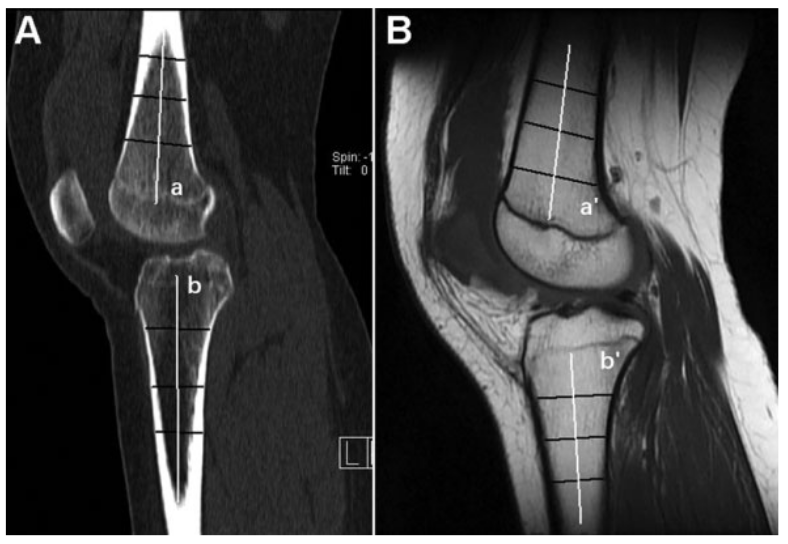
\includegraphics[width=0.7\linewidth]{dai_image}
	\caption{Femur and Tibia shaft axes defined in CT and T1-weighted MRI scans in the sagital view. \parencite{dai_comparing_2021}}
	\label{fig:daiimage}
\end{figure}

Interestingly, despite the observed angles suggesting a slight hyperextension, there was no significant difference in the angles between the loaded and unloaded conditions. This indicates that the loading condition did not significantly affect the alignment of the femur and tibia as measured by the angle between their long axes.

\subsection{Distance calculation}

Figure \ref{fig:resultsdistancestickman} shows the variation in the Euclidean distance between anatomical landmarks on the femur and tibia throughout the flexion-extension cycle. Initially, this distance decreases as the knee moves from a flexed to an extended position. In the second half of the cycle, the distance increases as the knee returns to the flexed position.

Significant differences were observed in the bins (0.0, 10.0] and (10.0, 20.0] with P-values of 0.022 and 0.015 under loaded conditions. This suggests that external loading affects the spatial relationship between the femur and tibia, but only during the beginning of the flexion phase. 

This effect may be due to the different types of muscle contractions during flexion and extension. The quadriceps, which cover most of the anterior and sides of the femur, contract either concentrically (shortening under tension) or eccentrically (lengthening under tension). During extension, the quadriceps contract concentrically to lift the leg against gravity. During flexion, they control the rate of knee bending under gravity \parencite{dalley_moores_2023}.

Since eccentric contractions generate higher force as compared to concentric contractions, they can be more susceptible to external loads \parencite{nuzzo_eccentricconcentric_2023}. This suggests that the influence of external loading is dependent on the type of muscle contraction. During extension, concentric contractions of the quadriceps provide a more stable form of contraction, and thus, the impact of external loading is not significant. In contrast, during flexion, the eccentric contractions are more susceptible to changes due to external loading. A previous study also observed load-dependent variations in tibiofemoral kinematics, which supports this finding \parencite{westphal_load-dependent_2013}.

Furthermore, the effect of external loading is primarily seen in the initial phase of flexion, particularly within the first few degrees of the flexion phase. This observation aligns with the findings of Fuchs et al. \parencite{fuchs_-vivo_2022}, who noted minimal torsional movement in the knee at this range of motion. Fuchs et al. chose 20 degrees of flexion as the 'extended' portion due to the anatomical constraints that limit torsional movement below this degree of flexion. This lack of torsional movement could explain why external loading significantly affects the femur-tibia spatial relationship only in the first few degrees of flexion observed in our study. As the knee begins to flex from a fully extended position, it experiences different biomechanical conditions compared to other phases of the cycle, making it more susceptible to external loads. Beyond this initial phase, the knee joint stabilizes, reducing the impact of external loading on the distance between femoral and tibial landmarks.



\section{Conclusion}
This study aimed to evaluate the biomechanical parameters of the knee joint during flexion-extension cycles under loaded and unloaded conditions using dynamic MRI scans. By implementing an edge tracking and segmentation algorithm, the study successfully semi-automated the extraction of these parameters from 2D cine images, providing a foundation for further analysis and potential clinical applications.

The edge tracking algorithm demonstrated reliable performance, with mean alignment errors per point comparable to established methods. This accuracy is crucial for ensuring precise segmentation of the tibia and femur, thereby enabling accurate measurements of biomechanical parameters. The method's reliability supports its use in effectively analyzing knee joint mechanics.

The analysis of biomechanical parameters revealed significant insights into knee joint behavior under different conditions. The Euclidean distance between anatomical landmarks on the femur and tibia showed significant differences in the early phase of flexion under loaded conditions, suggesting that external loading primarily affects the spatial relationship between these bones during eccentric muscle contraction phases. This highlights the complex interplay between muscle contraction types and external loading in influencing knee joint biomechanics.

The methods developed in this study can be used to semi-automate the segmentation of 2D cine images of the knee during flexion-extension motion cycles. This automation facilitates the extraction of biomechanical parameters, which are crucial for assessing joint health. Patients with osteoarthritis (OA) exhibit varying degrees of abnormal tibiofemoral kinematics compared to healthy individuals, as evidenced by research indicating that OA leads to significant changes in knee joint mechanics (e.g., altered joint contact mechanics and increased instability). The baseline measurements obtained from this study can serve as a reference for comparing kinematic differences in OA patients, aiding in the diagnosis and monitoring of the disease.


Extending this methodology to 3D imaging is a promising avenue for future research. By eliminating the issue of through-plane motion, 3D imaging can potentially lead to more accurate and comprehensive segmentation of the knee joint, thereby improving the precision of biomechanical parameter extraction. This advancement could significantly enhance the ability to study and understand knee joint mechanics in various conditions, including OA and other musculoskeletal disorders.

In conclusion, this study demonstrates the feasibility and utility of using dynamic MRI scans combined with advanced segmentation algorithms to analyze knee joint biomechanics. The findings provide a solid foundation for further research and clinical applications, with the potential to improve diagnostic and therapeutic approaches for knee joint disorders.

% ----------------------------------------------------------------------------
% Bibliography
% ----------------------------------------------------------------------------
\cleardoublepage
\phantomsection
\addcontentsline{toc}{section}{\refname} % to add Bibliography to toc
\printbibliography

% --------------------------
\cleardoublepage
\begin{appendix}
\section{Appendix}
If needed for supplementary material, such as detailed description of data collection, tables, or figures.

\end{appendix}

% ----------------------------------------------------------------------------
% Statutory declaration
% ----------------------------------------------------------------------------
\makeThesisDeclaration

\end{document}

